\documentclass[letterpaper,twocolumn,10pt]{article}
\usepackage{usenix,epsfig,endnotes}
\usepackage{amssymb}
\usepackage{amsthm}
\usepackage{enumitem}
\usepackage{tabularx}
\usepackage{boxedminipage}
\usepackage[override]{cmtt}
\usepackage[utf8]{inputenc}
\usepackage{color,xcolor}
\usepackage{graphicx}
\usepackage{xspace}
\usepackage{amsmath,amstext,amssymb,amsfonts,latexsym}
\usepackage{url,hyperref}
\usepackage{setspace}

\usepackage{tikz}
\usetikzlibrary{arrows,calc,fit,positioning,shapes.misc}

\pgfdeclarelayer{background}
\pgfsetlayers{background,main}

\tikzset{%
  entity/.style={rectangle,draw=black,align=center},
  trusted/.style={fill=green!30},
  communication/.style={blue},
  comm-link/.style={communication,ultra thick,text=black},
  bg-box/.style={rectangle,rounded corners,draw=black,dashed},
  blockchain-color/.style={fill=yellow!25},
  tc-server-color/.style={fill=black!20}
}

\DeclareMathAlphabet{\mathcal}{OMS}{cmsy}{m}{n}

\newcommand{\kyle}[1]{\textcolor{blue}{[\textsf{Kyle:  #1}]}}
\newcommand{\fan}[1]{\textcolor{red}{[\small \bf {Fan:  #1}]}}
\definecolor{darkgreen}{rgb}{0,0.6,0}
\newcommand{\ari}[1]{\textcolor{darkgreen}{[\textsf{Ari:  #1}]}}
\newcommand{\ethan}[1]{\textcolor{cyan}{[\textsf{Ethan: #1}]}}
\newcommand{\elaine}[1]{\textcolor{magenta}{[\textsf{elaine:  #1}]}}

% Complex \xxx for making notes of things to do.  Use \xxx{...} for general
% notes, and \xxx[who]{...} if you want to blame someone in particular.
% Puts text in brackets and in bold font, and normally adds a marginpar
% with the text ``xxx'' so that it is easy to find.  On the other hand, if
% the comment is in a minipage, figure, or caption, the xxx goes in the text,
% because marginpars are not possible in these situations.
{\makeatletter
 \gdef\xxxmark{%
   \expandafter\ifx\csname @mpargs\endcsname\relax % in minipage?
     \expandafter\ifx\csname @captype\endcsname\relax % in figure/caption?
       \marginpar{\textcolor{red}{xxx~}}% not in a caption or minipage, can use marginpar
     \else
       \textcolor{red}{xxx~}% notice trailing space
     \fi
   \else
     \textcolor{red}{xxx~}% notice trailing space
   \fi}
 \gdef\xxx{\@ifnextchar[\xxx@lab\xxx@nolab}
 \long\gdef\xxx@lab[#1]#2{{\bf \small [\xxxmark \textcolor{red}{#2} ---{\sc #1}]}\xspace}
 \long\gdef\xxx@nolab#1{{\bf \small [\xxxmark \textcolor{red}{#1}]}\xspace}
}

\newtheorem{lemma}{Lemma}
\newtheorem{definition}{Definition}
\newtheorem{theorem}{Theorem}

%don't want date printed
\date{}

%make title bold and 14 pt font (Latex default is non-bold, 16 pt)
\title{\Large \bf Town Crier: \\ An Authenticated Data Feed for Smart Contracts}

%for single author (just remove % characters)
\author{
{\rm Your N.\ Here}\\
Your Institution
\and
{\rm Second Name}\\
Second Institution
\and
{\rm Name}\\
Name Institution
} % end author


%**** COLORS *********
\definecolor{maroon}{RGB}{178, 34, 34}
%\definecolor{brown}{RGB}{139, 137, 137}
\definecolor{gold}{rgb}{0.85, 0.65, 0.13}

\newcommand{\smaroon}[1]{{\ensuremath{\tt {\color{maroon} #1}\xspace}}}
\newcommand{\sgold}[1]{\ensuremath{\tt {\color{gold} #1 \xspace}}}
\newcommand{\sbrown}[1]{\ensuremath{\tt {\color{brown} #1 \xspace}}}

\newcommand{\sgray}[1]{{\color{gray} #1}}

%**** DEFINITIONS *********

\newcommand {\tcs} {Town Crier\xspace}
\newcommand {\tc} {TC\xspace}
\newcommand {\tcontract} {{TC Contract}\xspace}
\newcommand {\encname} {{Enclave}\xspace}
\newcommand {\medname} {{Relay}\xspace}
\newcommand {\Time} {{{\tt T}}}


\newcommand {\reqcont} {\ensuremath{{\cal C}_U}\xspace}
\newcommand {\tcont} {\ensuremath{{\cal C}_{TC}}\xspace}
\newcommand {\tcadd} {\ensuremath{{\cal P}_{TC}}\xspace}
\newcommand {\pTC} {\ensuremath{{\cal P}_{TC}}\xspace}
\newcommand {\cont} {\ensuremath{{\cal C}}\xspace}
\newcommand {\sgxadd} {${\cal P}_{SGX}$\xspace}
\newcommand{\pkTC}{\ensuremath{{\sf pk}_{TC}}\xspace}
%\newcommand{\pkTC}{\ensuremath{{{\cal P}_{TC}.{\sf pk}}}\xspace}
%\newcommand{\skTC}{\ensuremath{{{\cal P}_{TC}.{\sf sk}}}\xspace}
\newcommand{\skTC}{\ensuremath{{\sf sk}_{TC}}\xspace}
%\newcommand{\skTC}{\ensuremath{{\sf sk}_{\textrm{TC}}}\xspace}

\newcommand {\dgreq} {{\sf req}\xspace}
\newcommand {\dgform} {{\sf params}\xspace}
\newcommand {\dgspec} {{\sf spec}\xspace}
\newcommand {\dgpay} {{\sf \$fee}\xspace}
\newcommand {\dg} {{\sf d}\xspace}
\newcommand {\dgret} {{\sf ans}\xspace}
\newcommand {\dgm} {{\sf data}\xspace}
\newcommand {\dgi} {{\sf d_{\mbox{$i$}}}\xspace}
\newcommand {\dgid} {{\sf id}\xspace}
\newcommand {\dgcallback} {{\sf callback}\xspace}

\newcommand {\att} {{\sf att}\xspace}

\newcommand{\fsgx}{\ensuremath{\mathcal{F}_{\textrm{sgx}}}\xspace}
\newcommand{\pk}{\ensuremath{{\sf pk}}}
\newcommand{\sk}{\ensuremath{{\sf sk}}}
\newcommand{\pkM}{\ensuremath{{\sf pk}_{\mathrm{sgx}}}}
\newcommand{\skM}{\ensuremath{{\sf sk}_{\mathrm{sgx}}}}
\newcommand{\pkU}{\ensuremath{{\sf pk}_{\mathcal{U}}}}
\newcommand{\pU}{\ensuremath{{\mathcal{P}}_{\mathcal{U}}}}
%\newcommand{\pksgx}{\ensuremath{{\mathcal{P}}_{\text{TC}}.{\sf pk}}}
\newcommand{\pksgx}{\ensuremath{{\sf pk}_{\textrm{TC}}}\xspace}
\newcommand{\sksgx}{\ensuremath{{\sf sk}_{\textrm{TC}}}\xspace}
\newcommand{\pkurl}{\ensuremath{{\sf pk}_{\textrm{url}}}\xspace}
\newcommand{\rl}{\ensuremath{{\sf RL}}}
\newcommand{\relay}{\ensuremath{\mathcal{R}}\xspace}
\newcommand{\engine}{\ensuremath{\enclaveprog}\xspace}
%\newcommand{\digest}{\ensuremath{{\sf digest}}}
\newcommand{\enclaveprog}{\ensuremath{{\sf prog}_{\textrm{encl}}}\xspace}
\newcommand{\prog}{\ensuremath{{\sf prog}}\xspace}
\newcommand{\sigatt}{\ensuremath{{\sigma_{\textrm{att}}}}\xspace}
\newcommand{\sigsgx}{\ensuremath{{\Sigma_{\textrm{sgx}}}}}
\newcommand{\weburl}{\ensuremath{{{\sf url}}}\xspace}
\newcommand{\clock}{\ensuremath{{{\sf clock}}}}
\newcommand{\algA}{\ensuremath{\mathcal{A}}}
\newcommand{\algB}{\ensuremath{\mathcal{B}}}

\newcommand{\initcall}{\texttt{init}\xspace}
\newcommand{\attcall}{\texttt{attest}\xspace}
\newcommand{\resumecall}{\texttt{resume}\xspace}

\newcommand{\gas}{\sbrown{\$G}}
\newcommand{\constgasmin}{\sbrown{\$\overline{G}_\text{min}}}
\newcommand{\constgasmax}{\sbrown{\$\overline{G}_\text{max}}}
\newcommand{\constgascancel}{\sbrown{\$\overline{G}_\emptyset}}
\newcommand{\gasdeliver}{\sbrown{\$G_\text{deliver}}}
\newcommand{\gasrequest}{\sbrown{\$G_\text{request}}}
\newcommand{\gascancel}{\sbrown{\$G_\text{cancel}}}
\newcommand{\fee}{\smaroon{\$F}}
\newcommand{\feecancel}{\smaroon{\$F_\emptyset}}


%*****************************

\begin{document}

\maketitle

% Use the following at camera-ready time to suppress page numbers.
% Comment it out when you first submit the paper for review.
% \thispagestyle{empty}

\begin{abstract}
Smart contracts are programs that execute autonomously on blockchains. Their key envisioned uses (e.g., financial instruments) require them to consume data from outside the blockchain (e.g., stock quotes). Trustworthy {\em data feeds} that can support a broad range of data requests will thus be critical to smart contract ecosystems. 

	We present an authenticated data feed system called {\em Town Crier} (TC). TC acts as a bridge between existing web sites, which are already commonly trusted for non-blockchain applications, and smart contracts. It combines a blockchain front end with a trusted hardware back end to scrape HTTPS-enabled websites and serve source-authenticated data to relying smart contracts. TC also supports confidentiality: It enables private data requests with encrypted parameters, as well as secure use of user credentials to scrape access-controlled online data sources.
	
	We describe TC's design principles and architecture and report on an implementation that uses Intel's recently introduced Software Guard Extensions (SGX) to furnish data to the Ethereum smart contract system. We formally model TCand  define and prove its basic security properties in the Universal Composibility (UC) framework. Our results include definitions and techniques of general interest relating to resource consumption (Ethereum's ``gas'' fee system) and TCB minimization. We also report on experiments with three example applications. 
	
	We plan to launch TC soon as an online public service.
\end{abstract}
\elaine{TODO: change $pk_{TC}$ notation. right now it is inconsistent throughout the paper}

\section{Introduction}

Smart contracts are computer programs that autonomously facilitate or execute a contract. For decades, they have been envisioned as a means to extend the reach of existing contract law and render it more precise and efficiently executable through logical specification of legal agreements. Szabo, who coined the term ``smart contact'' in a seminal 1993 paper~\cite{}, gave as an example a smart contract that enforces car loan payments. If the owner of the car fails to make a timely payment, a smart contract could revoke physical access and return control of the ignition key to the bank. The contract could additionally be programmed to do so only at a time that is safe for the the owner, e.g., while the car is parked.

The emergence of decentralized cryptocurrencies such as Bitcoin has created new opportunities to realize smart contracts, thanks to two properties. First, cryptocurrencies equate control of their assets with knowledge of a private cryptographic key, in principle making control of money possible by an arbitrary computer program such as a smart contract. Second, cryptocurrencies are built atop blockchains, whose state evolves through a consensus protocol that treats transactions as computations over a global data structure. As these computations are decentralized, a blockchain may be viewed as an idealized abstraction equivalent to a trusted third party. It ensures fair, automated execution of computations over global state and eliminates the need for trusted intermediaries. 

While the scripting language embodied in Bitcoin is intentionally limited (e.g., lacks support for loops), the recently launched decentralized cryptocurrency Ethereum supports Turing-complete code. Ethereum can thus in principle realize fully expressive, self-enforcing, and self-executing smart contracts, going a long way toward fulfilling the vision of researchers and proponents.  

As Szabo's example shows, though, the most compelling applications of smart contracts cannot be realized in isolation on a blockchain, but require access to data about real-world state and phenomena. Financial contracts and derivatives, perhaps the most commonly cited applications of Ethereum~\cite{}, must be able to consume data about financial markets, including equity and commodity prices and exchange rates. Applications such as insurance policies are only realizable with data about weather, flights, delivery of goods, and so forth. 

To meet this need, the architects of Ethereum have proposed the use of \emph{data feeds} (sometimes called ``oracles''), contracts on the blockchain that serve data requests by other contracts~\cite{whitepaper,yellowpaper}. A few such data feeds, such as PriceFeed and Oraclize.it, support Ethereum smart contracts today, but have a notable drawback: They provide no assurance of trustworthy data beyond the reputation of their operators (who are typically individuals or small entities), even if their is data ultimately obtained from trustworthy sources.\footnote{Oraclize.it itself makes use of TLSnotary to notarize data, thereby distributing trust across two (small) operators.\ari{I think TLSnotary just signs webpages. So it's not clear how the mapping from pages to data is authenticated.}} To address this problem, systems such as SchellingCoin and Augur~\cite{} have been proposed that rely on mechanisms such as prediction markets to decentralize trust. While decentralization of trust is attractive, and underpins cryptocurrencies to begin with, prediction markets can support only a limited number of data feeds and have not yet seen widespread use in cryptocurrencies. The lack of a substantive ecosystem of trustworthy data feeds in Ethereum indeed remains a critical obstacle to its evolution~\cite{???}.

At the same time, however, existing e-commerce already relies on a wealth of broadly trusted data available from existing sources, namely websites operated by generally reputable organizations. The sources of such data, moreover, can be authenticated by a client if served over HTTPS. Smart contracts, however, cannot directly access internet data, as they do not have network access.

We present a system called \emph{Town Crier} (\tc) that fills the gap between smart contracts and today's data sources by serving as what we call an \emph{authenticated data feed} (ADF). \tc functions as a bridge between existing HTTPS-enabled data sources and the Ethereum blockchain, retrieving data from these sources and serving it to relying contracts on the blockchain in the form of specific data items that we call \emph{datagrams}. \tc avoids the problem of bootstrapping trust by executing its core functionality in an environment protected by \emph{trusted hardware}. Specifically, \tc makes use of Intel's recently released Software Guard Instructions (SGX). SGX enables a server to run a piece of code $\prog$ in an isolated environment called an \emph{enclave} (protected against even a malicious OS) and \emph{attest} (prove) to a remote party that the party is interacting with a legitimate, SGX-backed instance of $\prog$. 

By operating through a smart-contract front end, \tc can thus furnish a requested datagram $X$ from a particular trusted source, e.g., \texttt{https://www.Y.com}, such that a relying contract $\cont$ can authenticate that $X$ came from $Y$ assuming only that: (1) $\prog$ correctly retrieves and serves data and (2) The \tc server's hardware has not been tampered with. (Of course, there is also a need to trust Intel, which serves as a root of trust for SGX-enabled hosts in general.) Note that trust in $Y$ itself is orthogonal, and \tc can combine data sources according to any desired policy (e.g., majority voting across sources).

While conceptually simple, \tc presents a number of technical challenges. First, there are implementation challenges in securely interfacing enclave code with the blockchain and with data sources. Ethereum lacks native support for and therefore does not permit efficient on-chain verification of the proprietary digital signatures SGX uses to generate attestations on enclave code. Enclave code cannot directly scrape blockchain data and must instead rely on an untrusted process to retrieve correct blockchain data.\footnote{This problem cannot be solved by the obvious mechanism of digitally signing blockchain data: The blockchain is globally readable, and thus cannot store private keys, and running a blockchain client in the enclave would bloat the TCB in the enclave unacceptably.} Additionally, for enclave code to communicate securely with data sources, it must do so over HTTPS, yet enclave code in SGX does not control the host's network stack, which is instead controlled by the (potentially untrusted) OS. A second challenge is in the proofs of security for \tc. These proofs require harmonized formalism for SGX and smart contracts that existing work does not yet provide. Moreover, Ethereum requires expenditure of a currency-derived resource known as \emph{gas} to power contracts; thus proving the availability of \tc---a critical property for relying contracts---requires conventional analysis of data integrity coupled with a proof of sustainable gas expenditure. Finally, the use of \tc raises confidentiality challenges. Since blockchain state is globally readable, na\"{i}ve use of \tc would expose potentially sensitive datagram requests, e.g., an flight-insurance policy would publicly reveal the flight information of policyholders, and would render \tc vulnerable to traffic analysis on served data. Much of our contribution in the design of \tc involves addressing these challenges. 

Beyond merely serving publicly visible requests for generic data, \tc supports private datagram requests in which the request is encrypted and custom datagram requests in which the requested data comes from an access-controlled system, such as an individual user's account. Thus \tc can support a rich variety of smart contracts, as shown by our implementation of three example contracts: (1) A financial derivative (cash-settled put option) that requires stock ticker data; (2) A flight insurance contract that relies on private data requests about flight cancellations; and (3) A contract for exchanging currency in an online role playing game for ether, the Ethereum currency, using custom data requests.

In summary, our contributions are as follows:

\vspace{-1mm}
\begin{itemize}
  \setlength{\itemsep}{2pt}
  \setlength{\parskip}{0pt}
  \setlength{\parsep}{0pt}

\item \emph{\tcs system:} We present and describe our implementation of \tc, an authenticated data feed system that enables smart contracts to obtain datagrams safely from a target data source, specifically an existing HTTPS-enabled server. In contrast to currently available systems, \tc's assurances do not require trust in (typically fledgling) service operators, only in the underlying commodity trusted hardware, namely Intel SGX. 

\item \emph{Interfacing SGX with smart contracts:} We present solutions to the technical challenges that arise in combining two new technologies with incompatible APIs, e.g., the lack of Ethereum support for SGX attestations and the impracticality of authenticating blockchain data, and thus datagram requests, to \tc's trusted enclave program. 

\item \emph{\tc security analysis:} We present unifying formalism for the trusted hardware and smart contracts embodied in \tc and provide proofs of security, including the integrity and source authenticity of datagrams and service availability, which requires a new form of analysis of sustainable gas consumption. 

\item \emph{\tc applications:} We implement three practical smart contract applications that benefit from \tc: a financial derivative, a flight insurance contract, and a contract for exchanging online game currency and cryptocurrency. These applications showcase the rich possibilities and capabilities of \tc, including support for private and custom datagrams. 

\end{itemize}

As \tc has minimal trust assumptions and requires no modification to existing data source servers or Ethereum, we believe it offers a compelling, practical approach to bootstrapping a data feed ecosystem for smart contracts.



%\vspace{-3mm}
\section{Background}
\label{sec:background}

In this section, we provide basic background respectively on the main technologies \tc incorporates, namely SGX, TLS / HTTPS, and smart contracts.

%\vspace{-2mm}
\paragraph{\bf SGX.}
Intel's Software Guard Extensions (SGX)~\cite{sgx,sgxfordummy,mckeen2013sgx,anati2013sgx,hoekstra2013sgx} is a set of new instructions that confer hardware protections on user-level code. SGX enables a process to execute in a protected address space known as an {\em enclave}, which protects the confidentiality and integrity of the process from other software on the same host, including the operating system, and certain forms of hardware attack. 

A enclave process cannot make system calls, but can read and write memory outside the enclave region. Thus isolated execution in SGX may be viewed in terms of an ideal model in which a process is guaranteed to execute correctly and with perfect confidentiality, but relies on a (potentially malicious) operating system for network and file-system access.\footnote{This model is a simplification: SGX is known to expose some internal enclave state to the OS~\cite{sgxexplained}. Our basic security model for \tc assumes ideal isolated execution, but again, \tc can also be distributed across multiple SGX instances as a hedge against compromise.}

SGX allows a remote system to verify the software in an enclave and communicate securely with it. When an enclave is created, the CPU produces a hash of its initial state known as a {\em measurement}. The software in the enclave may at a later time request a report, which includes a measurement and supplementary data provided by the process, such as a public key. The report may be digitally signed using a hardware-protected key to produce a proof that the measured software is running in an SGX-protected enclave. This proof, known as a {\em quote}, may be verified by a remote system, while the process-provided public key can be used by the remote system to establish a secure channel with the enclave or verify signed data it emits. We use the generic term {\em attestation} to refer to a quote, and denote it by \att. We assume that a trustworthy measurement of the code for the enclave component of \tc is available to any client that wishes to verify an attestation. SGX signs quotes using a \emph{group signature} scheme called 
EPID~\cite{epid}. This choice of primitive is significant in our design of \tcs, as EPID is a proprietary signature scheme not supported in Ethereum.

SGX additionally provides a trusted time source via the function \texttt{sgx\_get\_trusted\_time}.~On invoking this function, an enclave obtains a measure of time relative to a reference point indexed by a nonce. A reference point remains stable, but SGX does not provide a source of absolute or wall-clock time, a limitation that we must work around in \tc.

%\vspace{-2mm}
\paragraph{\bf TLS / HTTPS.}
We assume basic familiarity by readers with TLS and HTTPS (HTTP over TLS). As we explain later, \tc exploits an important feature of HTTPS, namely that it can be partitioned into interoperable layers: An HTTP layer interacting with web servers, a TLS layer handling handshakes and secure communication, and a TCP layer providing reliable data stream. 

%\vspace{-2mm}
\paragraph{\bf Smart contracts.}
\label{sec:contracts-and-gas}
While \tc can in principle support any smart-contract system, we focus in this paper on its use in Ethereum, whose use we now explain. For further details, see~\cite{whitepaper,yellowpaper}

A smart contract in Ethereum is represented as what is called a \emph{contract account}, endowed with code, a currency balance, and persistent memory in the form of a key/value store. A contract accepts messages as inputs to any of a number of designated functions. These entry points, determined by the contract creator, represent the API of the contract. Once created, a contract executes autonomously; it persists indefinitely, with even its creator unable to modify its code.\footnote{There is one exception: A special opcode \texttt{suicide} wipes code from a contract account.} Contract code executes in response to receipt of a \emph{message} from another contract or a \emph{transaction} from a non-contract (\emph{externally owned}) account, informally what we call a \emph{wallet}. Thus, contract execution is always initiated by a transaction. Informally, a contract only executes when ``poked,'' and poking progresses through a sequence of entry points until no further message passing occurs (or a shortfall in gas occurs, as explained below). The ``poking'' model aside, as a simple abstraction, a smart contract may be viewed as an {\em autonomous agent} on the blockchain.

Ethereum has its own associated cryptocurrency called \emph{ether}. (At the time of writing, 1 ether has a market value of a little more than \$5 U.S. \cite{ethprice}.)  To prevent Denial-of-Service (DoS) attacks, inadvertent infinite looping within contracts, and generally to control network resource expenditure,
Ethereum allows ether-based purchase of a resource called \emph{gas} to power contracts.
Every operation, including sending data, executing computation, and storing data, has a fixed gas cost.
Transactions and messages include a parameter (\texttt{GASLIMIT}) specifying a bound on the amount of gas expended by the computations they initiate.
When a function call is made, the child function expends gas from the same source as the parent function.
Should a function fail to complete due to a gas shortfall,
it is aborted and any state changes induced by the partial computation are rolled back to their pre-call state;
previous computations on the call path, though, are retained.

Along with a \texttt{GASLIMIT}, a transaction specifies a \texttt{GASPRICE}, the maximum amount in ether that the transaction is willing to pay per unit of gas. The transaction thus succeeds only if the initiating account has a balance of \texttt{GASLIMIT} $\times$ \texttt{GASPRICE} ether and \texttt{GASPRICE} is high enough to be accepted by the system (miner). 

The management of gas, as we show in our design of \tcs can be delicate. Without careful construction, \tc's smart contract front end on the Ethereum blockchain can be caused by an attacker to exhaust the ether used to power the delivery of datagrams.

Finally, we note that transactions in Ethereum are digitally signed for a wallet using ECDSA on the curve Secp256k1 and the hash function SHA3-256.




 \section{\tc Architecture and Security Model}

%In this section, we discuss the general design of \tc. First we present a strawman system design that illustrates some of the technical challenges that arise in the design of \tc. We then present our \tc architecture, describing the front-end (blockchain) and back-end (off-chain) components, and give a high-level view of the security model underpinning our design.

\iffalse{
\subsection{Strawman design}

Here we sketch a simple (but, as we show, na\"{i}ve) strawman design that provides authenticated data feeds along with accompanying attestations. 

%To harmonize with terminology introduced shortly in the paper, we refer to the untrusted component of a \tc host as the \medname and the code running in an SGX enclave as the \encname.

The strawman solution is as follows:

\begin{itemize}[leftmargin=5mm]
\item
{\bf Monitor and relay.}
The \tc system
monitors the blockchain for 
datagram requests. A contract \reqcont 
requests a datagram by including a distinguished message in its state (e.g., ``\tc service \#123 request:''), along with
a specification \dgform of the requested datagram.
Monitoring happens in the untrusted part of the \tc server, which controls the network stack. Any scraped specification \dgform is passed to a (trusted) enclave process.
\item
{\bf Securely fetch feed.}
Based on the \dgform, the trusted enclave process contacts a data source, establishing an HTTPS channel to a suitable target web page $\weburl$ (which might, e.g., be specified in \dgform). 
The process verifies that the validity of the certificate for the host serving \weburl.
It then fetches page contents, parses them, and extracts a datagram \dgm as specified in \dgform.

Finally, the enclave process produces an attestation $\att$ on: its code in the enclave, $\dgform$, a timestamp $T$ on the fetched data, and $\dgm$. 
It sends $\att$ to $\reqcont$.
\item
{\bf Verify}.
\reqcont verifies the attestation $\att$. If successful, \reqcont consumes \dgm (potentially matching \dgform against an internal queue of datagram requests).
\end{itemize}

This strawman scheme has a few nice features: conceptual simplicity, no need to maintain a \tc contract on the blockchain, and the ability for \reqcont to check the freshness of \att. It has a few serious drawbacks, however.

\paragraph{Problems with the strawman scheme.}
Our strawman scheme is unworkable for several reasons. First, verification of \att in the requesting contract \reqcont is not practical. Although SGX provides a 
trusted clock, the clock does not provide absolute time, but only time relative to a host-specific reference point.
Thus it is not clear in our strawman scheme how to produce a timestamp $T$ in absolute time. Furthermore, in Ethereum, opcodes for in-contract cryptographic operations are very limited and do not support the proprietary EPID group-signature scheme present in SGX attestations. While achievable in principle, as the Ethereum virtual machine is Turing-complete, verification of attestations would impose prohibitively expensive gas costs on \reqcont. 

To address these problems, our \tc architecture supports only off-chain verification of attestations.

Another problem with our strawman scheme is that it lacks an on-blockchain mechanism to enforce payment for datagrams. It is desirable for \tc to accept payments via a smart contract in order to permit payment in the system's cryptocurrency (e.g., Ether) and to ensure a {\em fair exchange} between payments and datagrams. Even a not-for-profit \tc service might accept small gas payments to cover the cost of datagram transmission. Without enforcement of fair exchange, relying contracts or the \tc service would risk being defrauded by the other party. \tc could attempt to deliver datagrams only to contracts whose code guarantees payment to \tc, but verifying this property even in templated code would be challenging, given the many complicated dependencies in a smart-contract system (e.g., a contract might attempt to make payment but lack gas or ether). 

To address these problems, our \tc architecture uses a smart contract \tcont as a blockchain front end.
\fi

The \tcs system includes three main components: The \tcontract (\tcont), the \encname (\engine), and the \medname (\relay). The \encname and \medname reside on the \tc server, while the \tcontract  resides on the blockchain. An architectural schematic showing the roles of these components is given in Figure~\ref{fig:overview}.

\vspace{-2mm}
\begin{figure}[h!]
\centering
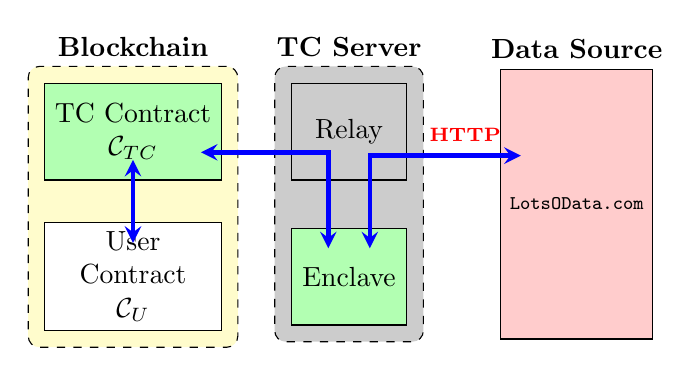
\begin{tikzpicture}
  [entity/.style={rectangle,draw=black,minimum height=3.5em,text width=3.5em,align=center},
   contract/.style={entity,text width=5.7em},
   trusted/.style={fill=green!30},
   communication/.style={blue,ultra thick,text=black},
   bg-box/.style={rectangle,rounded corners,draw=black,dashed}]
  \node[contract,trusted] (ctc) {TC Contract\\$\tcont$};
  \node[contract,fill=white,below=1.5em of ctc] (cu) {User Contract\\$\reqcont$};
  \node[entity,fill=none,right=2.5em of ctc] (relay) {Relay};
  \node[entity,trusted,right=2.5em of cu] (enc) {Enclave};

  \begin{pgfonlayer}{background}
    \node[bg-box,
          fill=yellow!20,
          fit={($(ctc.north east)+(0.25em,0.25em)$)($(cu.south west)+(-0.25em,-0.25em)$)},
          label=above:{\bf Blockchain}] (blockchain) {};
    \node[bg-box,
          fill=black!20,
          fit={($(relay.north east)+(0.25em,0.25em)$)($(enc.south west)+(-0.25em,-0.25em)$)},
          label=above:{\bf TC Server}] (tc) {};
  \end{pgfonlayer}

  \node[right=-0.15em of tc,color=red,transform canvas={yshift=2.5em}] (https) {\scriptsize \bf HTTPS};
  \node[rectangle,draw=black,fill=red!20,right=2.75em of tc,minimum height=9.75em,label=above:{\bf Data Source}] (data) {\scriptsize \tt LotsOData.com};

  \draw[stealth-stealth,communication] ([xshift=-0.75em,yshift=-0.75em]ctc.east) -| ([xshift=-0.75em,yshift=-0.75em]enc.north);
  \draw[stealth-stealth,communication] ([yshift=0.75em]ctc.south) -- ([yshift=-0.75em]cu.north);
  \draw[stealth-stealth,communication] ([xshift=0.75em,yshift=-0.75em]enc.north) |- ([xshift=0.75em,yshift=1.75em]data.west);
\end{tikzpicture}
\caption{{\bf Basic Town Crier architecture.}}
\label{fig:overview}
\end{figure}

%\begin{figure}[h!]
%\centering
%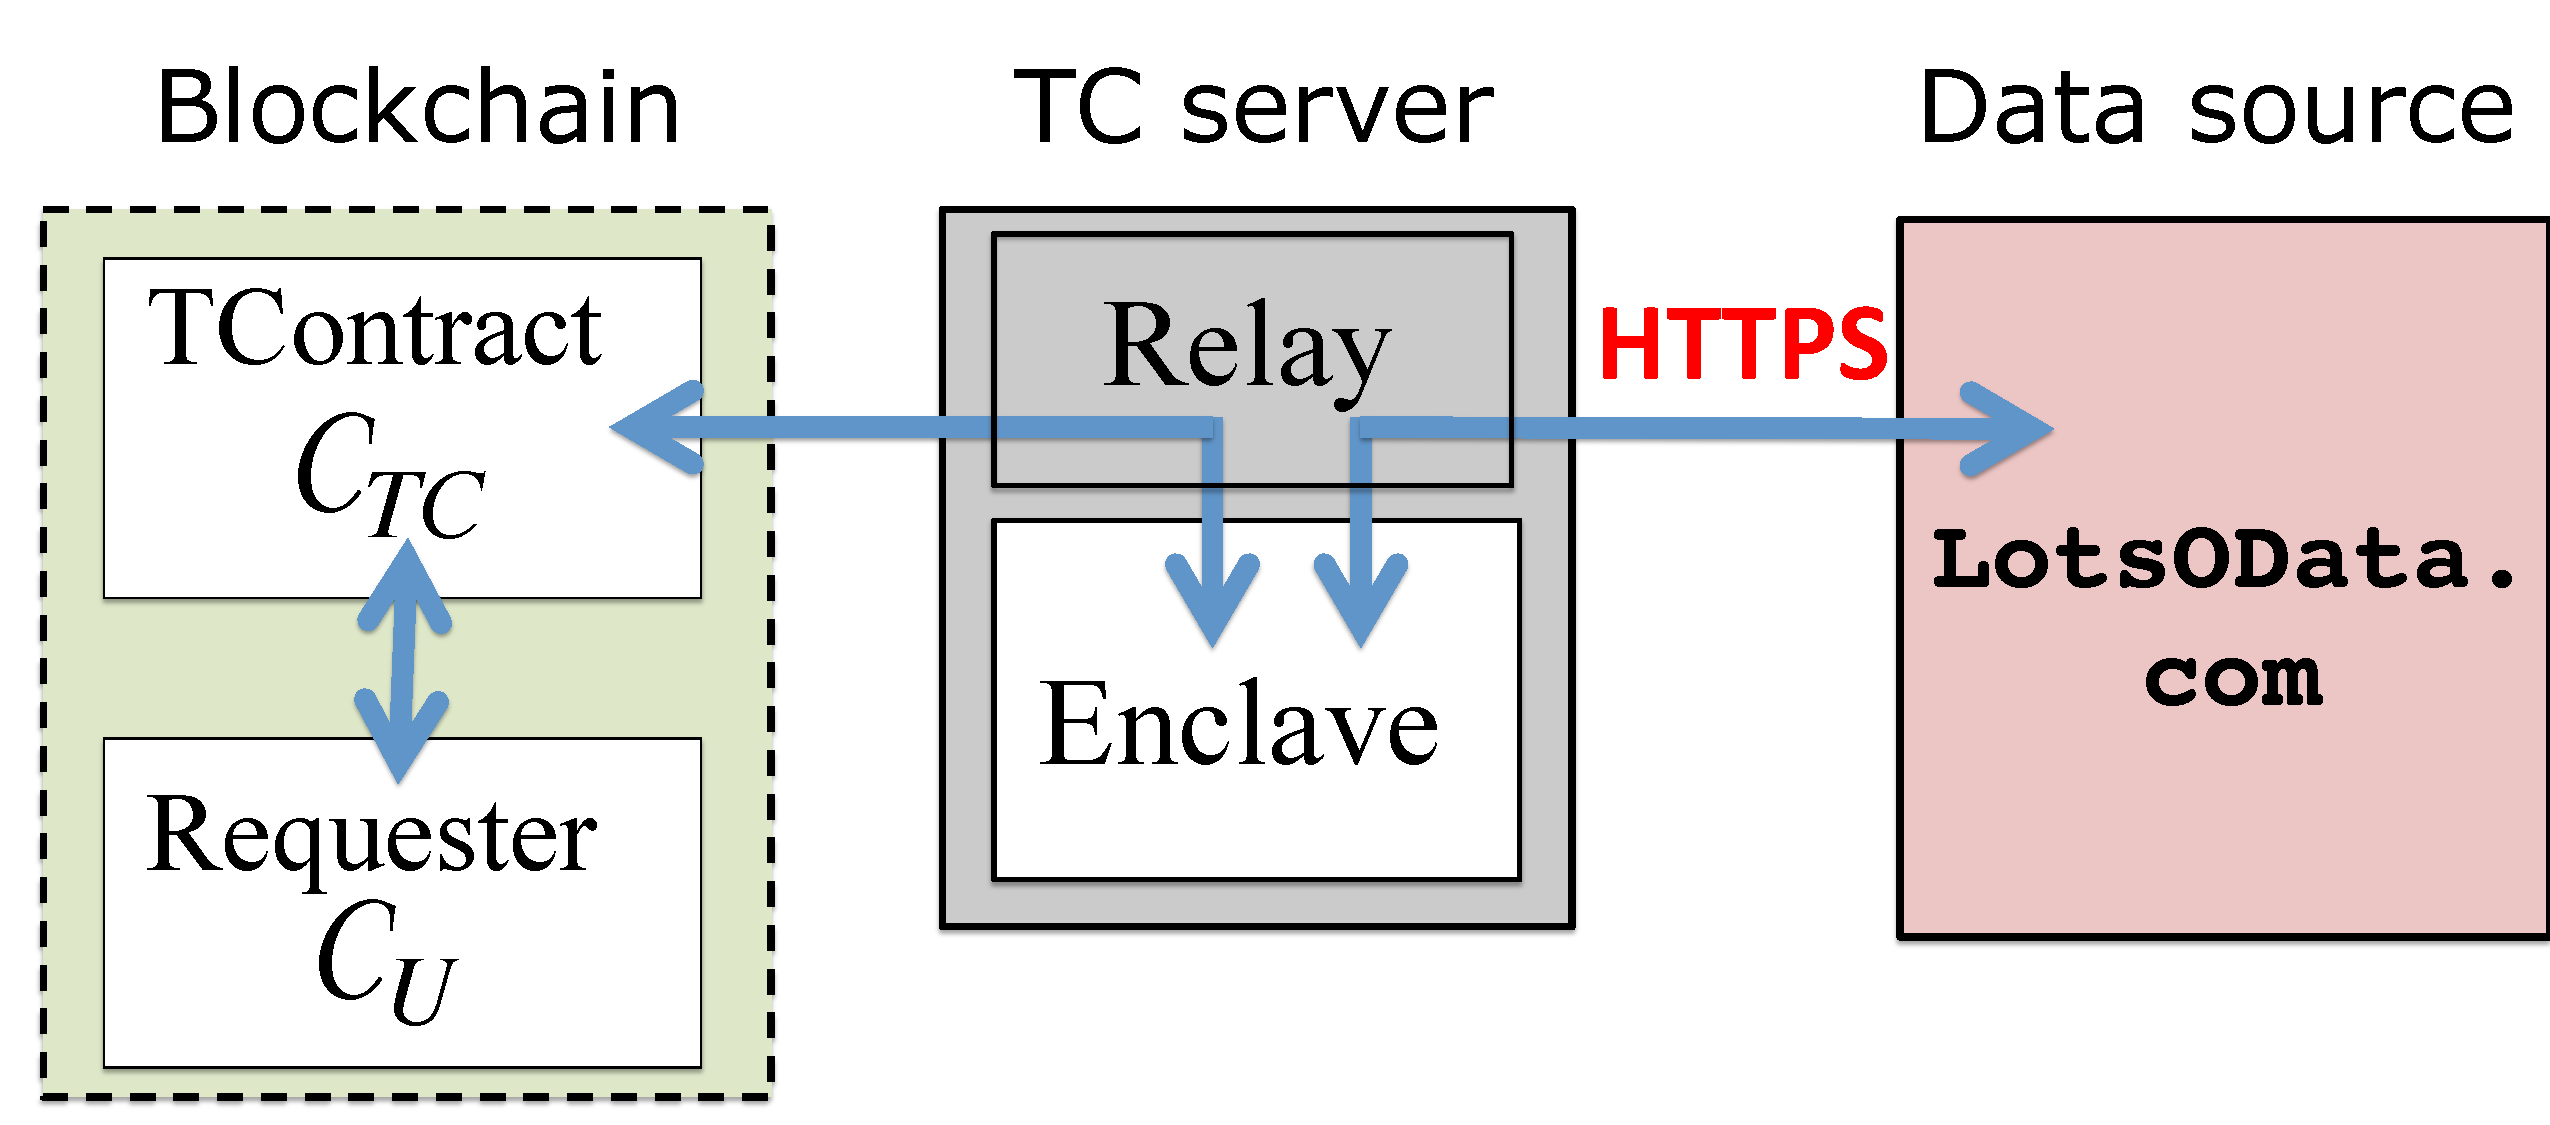
\includegraphics[width=\columnwidth]{figures/OverviewFig}
%\caption{{\bf Basic Town Crier architecture.}}
%\label{fig:overview}
%\end{figure}
\vspace{-2mm}

\paragraph{The \tcontract \tcont.} The \tcontract (denoted by \tcont) is a smart contract that acts as the blockchain front end of the \tc service. It is designed to present a simple API to a relying contract \reqcont for its requests from \tc. Very simply, \tcont accepts datagram requests from a requester \reqcont and returns corresponding datagrams from \tc. Additionally, \tcont manages \tc monetary resources, which in Ethereum take the form of ether (money) and gas (``fuel'' for contracts).

\paragraph{The \encname \engine.}
We refer to the TC code running in the SGX enclave simply as the \encname. In TC, the \encname ingests and fulfills datagram requests from the blockchain. To obtain the data for inclusion in datagrams, it queries external data sources, specifically HTTPS-enabled internet services. It returns a datagram to a requesting contract \reqcont as a digitally signed blockchain message. Under our assumed security model for SGX, apart from its network functions, the \encname runs in complete isolation from an adversarial OS as well as other process on the host. 

\paragraph{The \medname \relay.} As an SGX enclave process, the \encname lacks direct network access. Thus the \medname handles bidirectional network traffic on behalf of the \encname. Specifically, the \medname provides network connectivity from the \encname to three different types of entities: 

\begin{enumerate}
\item {\em The Blockchain (the Ethereum system):}  The \medname scrapes the blockchain in order to monitor the state of the \tcontract  \tcont. In this way, it performs implicit message passing from \tcont to the \encname, as neither component itself has network connectivity. Additionally, the \medname places messages emitted from the \encname (datagrams) on the blockchain.
\item {\em Clients:} The \medname runs a web server to handle off-chain service requests from clients, specifically, requests for attestations from the \encname. As we soon explain, an attestation provides a unique public key for the \encname instance to the  client and proves that the \encname is executing correct code in an enclave and that its clock is correct in terms of absolute (wall-clock time). A client that successfully verifies an attestation can then safely create a relying contract \reqcont that uses the \tc.
\item {\em Data sources:} The \medname relays traffic to and from data sources (HTTPS-enabled servers) queried by the \encname. 
\end{enumerate}

The \medname is an ordinary user-space application. It does not benefit from integrity protection by SGX and thus, unlike the \encname, can be subverted by an adversarial OS on the \tc server, causing network delays or failures. A key design aim of \tc, however, is that \medname should be unable to cause incorrect datagrams to be produced or users to lose fees paid to \tc for datagrams (although they may lose gas used to fuel their requests). As we shall show, in general the \medname~{\em can only mount denial-of-service attacks against \tc}. 

\paragraph{Security model}

Here we give a brief overview of our security model for \tc, providing more details in later sections. We assume the following:

\begin{itemize}

\item {\em Blockchain communication.} Transaction and message sources are authenticable, i.e., a transaction $m$ sent from an account ${\cal P}_{X}$ (or message $m$ from contract ${\cal C}_{X}$) is identified by the receiving account as originating from $X$. Transactions and messages are integrity protected (as they are digitally signed by the sender), but not confidential. 

\item {\em \encname security:} We make three assumptions about \encname : (1) The \encname behaves honestly, i.e., correctly executes the \tc protocol; (2) The private key $\skTC$ is known only to the \encname; and (3) The \encname has an accurate (internal) real-time clock. (Specifically, the clock is accurate to within \ari{XXX}, as we show experimentally.)  We explain in the next section how we achieve these properties through use of SGX and how the public key $\pkTC$ may be bound to an Ethereum account, given the \encname an authenticable blockchain presence. 

\item {\em Network communication.} The \medname (and other untrusted components of the \tc server) can tamper with or delay communications to and from the \encname. (As we explain in our SGX security model, the \medname cannot otherwise observe or alter the behavior of the \encname.) Thus the \medname is subsumed by an adversary that controls the network. 

\end{itemize}















\section{Basic \tc Protocol}
\label{sec:protocols}
We now describe the operation of \tc at the protocol level. The basic protocol is conceptually simple: a user contract \reqcont requests a datagram from the \tcontract \tcont, \tcont forwards the request to \engine and then returns the response to \reqcont. There are many details, however, relating to message contents and protection and the need to connect the off-chain parts of \tc with the blockchain.

First we give a brief protocol overview. Then we enumerate the data flows in \tc. Finally, we provide a component-level view of the protocol by specifying the operation of the \tcontract, \medname, and \encname. We present these  as ideal functionalities, inspired by the universal-composability (UC) framework, in order to abstract away implementation details and as a springboard for formal proofs of security. We omit details in this section on how payment is incorporated into \tc, deferring this delicate aspect of the system design to Section~\ref{sec:enhanced_protocol}.

\subsection{Datagram Lifecycle}

The lifecycle of a datagram may be briefly summarized in the following steps:

\vspace{-1ex}
\begin{itemize}
  \setlength{\itemsep}{2pt}
  \setlength{\parskip}{0pt}
  \setlength{\parsep}{0pt}
\item {\bf Initiate request.} \reqcont sends a datagram request to \tcont on the blockchain.

\item {\bf Monitor and relay.} The \medname monitors \tcont and relays any incoming datagram request with parameters \dgform to the \encname.

\item {\bf Securely fetch feed.} To process the request specified in \dgform, the \encname contacts a data source via HTTPS and obtains the requested datagram. It forwards the datagram via the Relay to \tcont.

\item {\bf Return datagram.} \tcont returns the datagram to \reqcont.
\end{itemize}
\vspace{-1ex}

\noindent We now make this data flow more precise. 

\subsection{Data Flows}
\label{sec:protocol-data-flows}

A datagram request by \reqcont takes the form of a message $m_1 = (\dgform, \dgcallback)$ to \tcont on the blockchain. $\dgform$ specifies the requested datagram, e.g., ${\sf params} := (\weburl, {\sf spec}, T)$, where $\weburl$ is the target data source, {\sf spec} specifies content of a the datagram to be retrieved (e.g., a stock ticker at a particular time), and $T$ specifies the delivery time for the datagram (initiated by scraping of the data source). The parameter $\dgcallback$ in $m_1$ indicates the entry point in \reqcont to which the datagram is to be returned. (In principle, $\dgcallback$ could point to a different contract, but \tc does not yet adopt this generalization.) 

\tcont generates a fresh unique $\dgid$ and forwards $m_2 = (\dgid, \dgform)$ to the \encname. It receives in return a return message $m_3 = (\dgid, \dgform, \dgm)$ from the \tc service, where $\dgm$ is the datagram (e.g., the desired stock ticker price). \tcont checks the consistency of $\dgform$ on the incoming and outgoing messages, and if they match forwards $\dgm$ to the entry point \dgcallback in \reqcont in message $m_4$.

For simplicity here, we assume that $\reqcont$ makes a one-time datagram request. Thus it can trivially match $m_4$ with $m_1$. Our full protocol contains an optimization by which $\tcont$ returns $\dgid$ to $\reqcont$ after $m_1$ as a consistent, trustworthy identifier for all data flows. This enables straightforward handling of multiple datagram requests from the same instance of $\reqcont$.

Fig.~\ref{fig:dataflow} shows the data flows involved in processing a datagram request. For simplicity, the figure omits the \medname, which is only responsible for data passing.


%\begin{figure}[h!]
%\centering
%\begin{tikzpicture}
%  [entity/.style={rectangle,draw=black,minimum height=3em,text width=6em,align=center},
%   trusted/.style={fill=green!30},
%   communication/.style={blue,ultra thick,text=black},
%   bg-box/.style={rectangle,rounded corners,draw=black,dashed},
%   blockchain-color/.style={fill=yellow!20}]
%  \node[entity,trusted,minimum height=4.5em] (ctc) {};
%  \node[entity,draw=none,anchor=north] (ctc-inner) at (ctc.north) {TC Contract\\$\tcont$~~~~~};
%  \node[entity,trusted,right=7em of ctc] (enc) {Enclave};
%  \node[entity,fill=white,below=5em of ctc,anchor=north west,xshift=1em] (cu) {User Contract\\$\reqcont$};
%  \node[entity,trusted,minimum height=1.5em,text width=3em,anchor=south west] (id-gen) at (ctc.south west) {\footnotesize $\dgid$ gen};
%
%  \draw[->,communication] ([yshift=-0.5em]cu.west) -| node [text width=3.3em,align=center,blockchain-color,yshift=3.5em] {\footnotesize $m_0 =$\\[-0.2em]$(\dgform,$\\[-0.2em]$\dgcallback)$} ([xshift=-2.4em]ctc.south);
%  \draw[->,communication,thick,dashed] ([xshift=-0.5em]ctc.south) |- node [text width=3em,xshift=1.5em,xshift=0.5em,yshift=3em] {\footnotesize $m_1 =$\\[-0.2em]$(\dgid)$} ([yshift=0.5em]cu.west);
%  \path[->,communication] (ctc) edge [above,transform canvas={yshift=0.6em}] node [text width=4em,align=center,xshift=-0.25em] {\footnotesize $m_2 =$\\[-0.4em]$(\dgid,\dgform)$} (enc);
%  \path[->,communication] (enc) edge [below,transform canvas={yshift=-0.6em}] node [text width=4em,align=center] {\footnotesize $m_3 =$\\[-0.2em]$(\dgid,\dgform,$\\[-0.3em]$\dgm)$} (ctc);
%  \draw[->,communication] ([yshift=-1.75em]ctc.east) -| node [text width=3em,align=center,blockchain-color,yshift=-3em] {\footnotesize $m_4 =$\\[-0.4em]$(\dgid,\dgm)$} (cu);
%
%  \path[->,green!40!black,text=black,ultra thick] ($(id-gen.east)+(-0.25em,0)$) edge [above right] node [xshift=0.25em,yshift=0.25em] {\footnotesize $\dgid$} ($(id-gen.east)+(1em,1em)$);
%
%  \begin{pgfonlayer}{background}
%    \node[bg-box,
%          blockchain-color,
%          fit={($(ctc.north west)+(-0.75em,0.25em)$)($(cu.south east)+(0.75em,-0.25em)$)},
%          label=above:{\bf Blockchain}] (bc-bg) {};
%    \node[bg-box,
%          fill=black!20,
%          fit={($(enc.north east)+(0.5em,1em)$)($(enc.south west)+(-0.5em,-1em)$)},
%          label=above:{\bf TC Server}] (tc-bg) {};
%  \end{pgfonlayer}
%  \node[below=0.4em of tc-bg,align=center] (data) {\small (obtains $\dgm$\\from data source)};
%\end{tikzpicture}
%\caption{{\bf Data flows in datagram processing.}}
%\label{fig:dataflow}
%\end{figure}

\begin{figure}[h!]
\centering
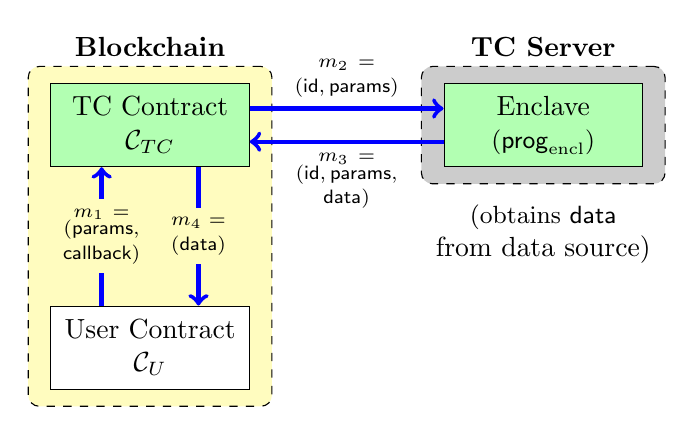
\begin{tikzpicture}
  [local-entity/.style={entity,minimum height=3em,text width=6.5em}]
  \node[local-entity,trusted] (ctc) {\tcontract\\$\tcont$};
  \node[local-entity,trusted,right=7em of ctc] (enc) {\encname\\{\small $(\enclaveprog)$}};
  \node[local-entity,fill=white,below=5em of ctc] (cu) {User Contract\\$\reqcont$};
  \node[below=1em of enc,align=center] (data) {\small (obtains $\dgm$\\from data source)};

  \path[->,comm-link] (cu) edge [transform canvas={xshift=-1.75em}] node [text width=3.5em,align=center,blockchain-color] {\scriptsize $m_1 =$\\[-0.2em]$(\dgform,$\\[-0.4em]$\dgcallback)$} (ctc);
  \path[->,comm-link] (ctc) edge [above,transform canvas={yshift=0.6em}] node [text width=4em,align=center] {\scriptsize $m_2 =$\\[-0.4em]$(\dgid,\dgform)$} (enc);
  \path[->,comm-link] (enc) edge [below,transform canvas={yshift=-0.6em}] node [text width=4em,align=center] {\scriptsize $m_3 =$\\[-0.2em]$(\dgid,\dgform,$\\[-0.4em]$\dgm)$} (ctc);
  \path[->,comm-link] (ctc) edge [transform canvas={xshift=1.75em}] node [text width=2.5em,align=center,blockchain-color] {\scriptsize $m_4 =$\\[-0.4em]$(\dgm)$} (cu);

  \begin{pgfonlayer}{background}
    \node[bg-box,
          blockchain-color,
          inner xsep=0.8em,
          inner ysep=0.6em,
          fit=(ctc)(cu),
          label=above:{\bf Blockchain}] () {};
    \node[bg-box,
          tc-server-color,
          inner xsep=0.8em,
          inner ysep=0.6em,
          fit=(enc),
          label=above:{\bf TC Server}] () {};
  \end{pgfonlayer}
\end{tikzpicture}
\caption{{\bf Data flows in datagram processing.}}
\label{fig:dataflow}
\end{figure}


%\begin{figure}[h!]
%\centering
%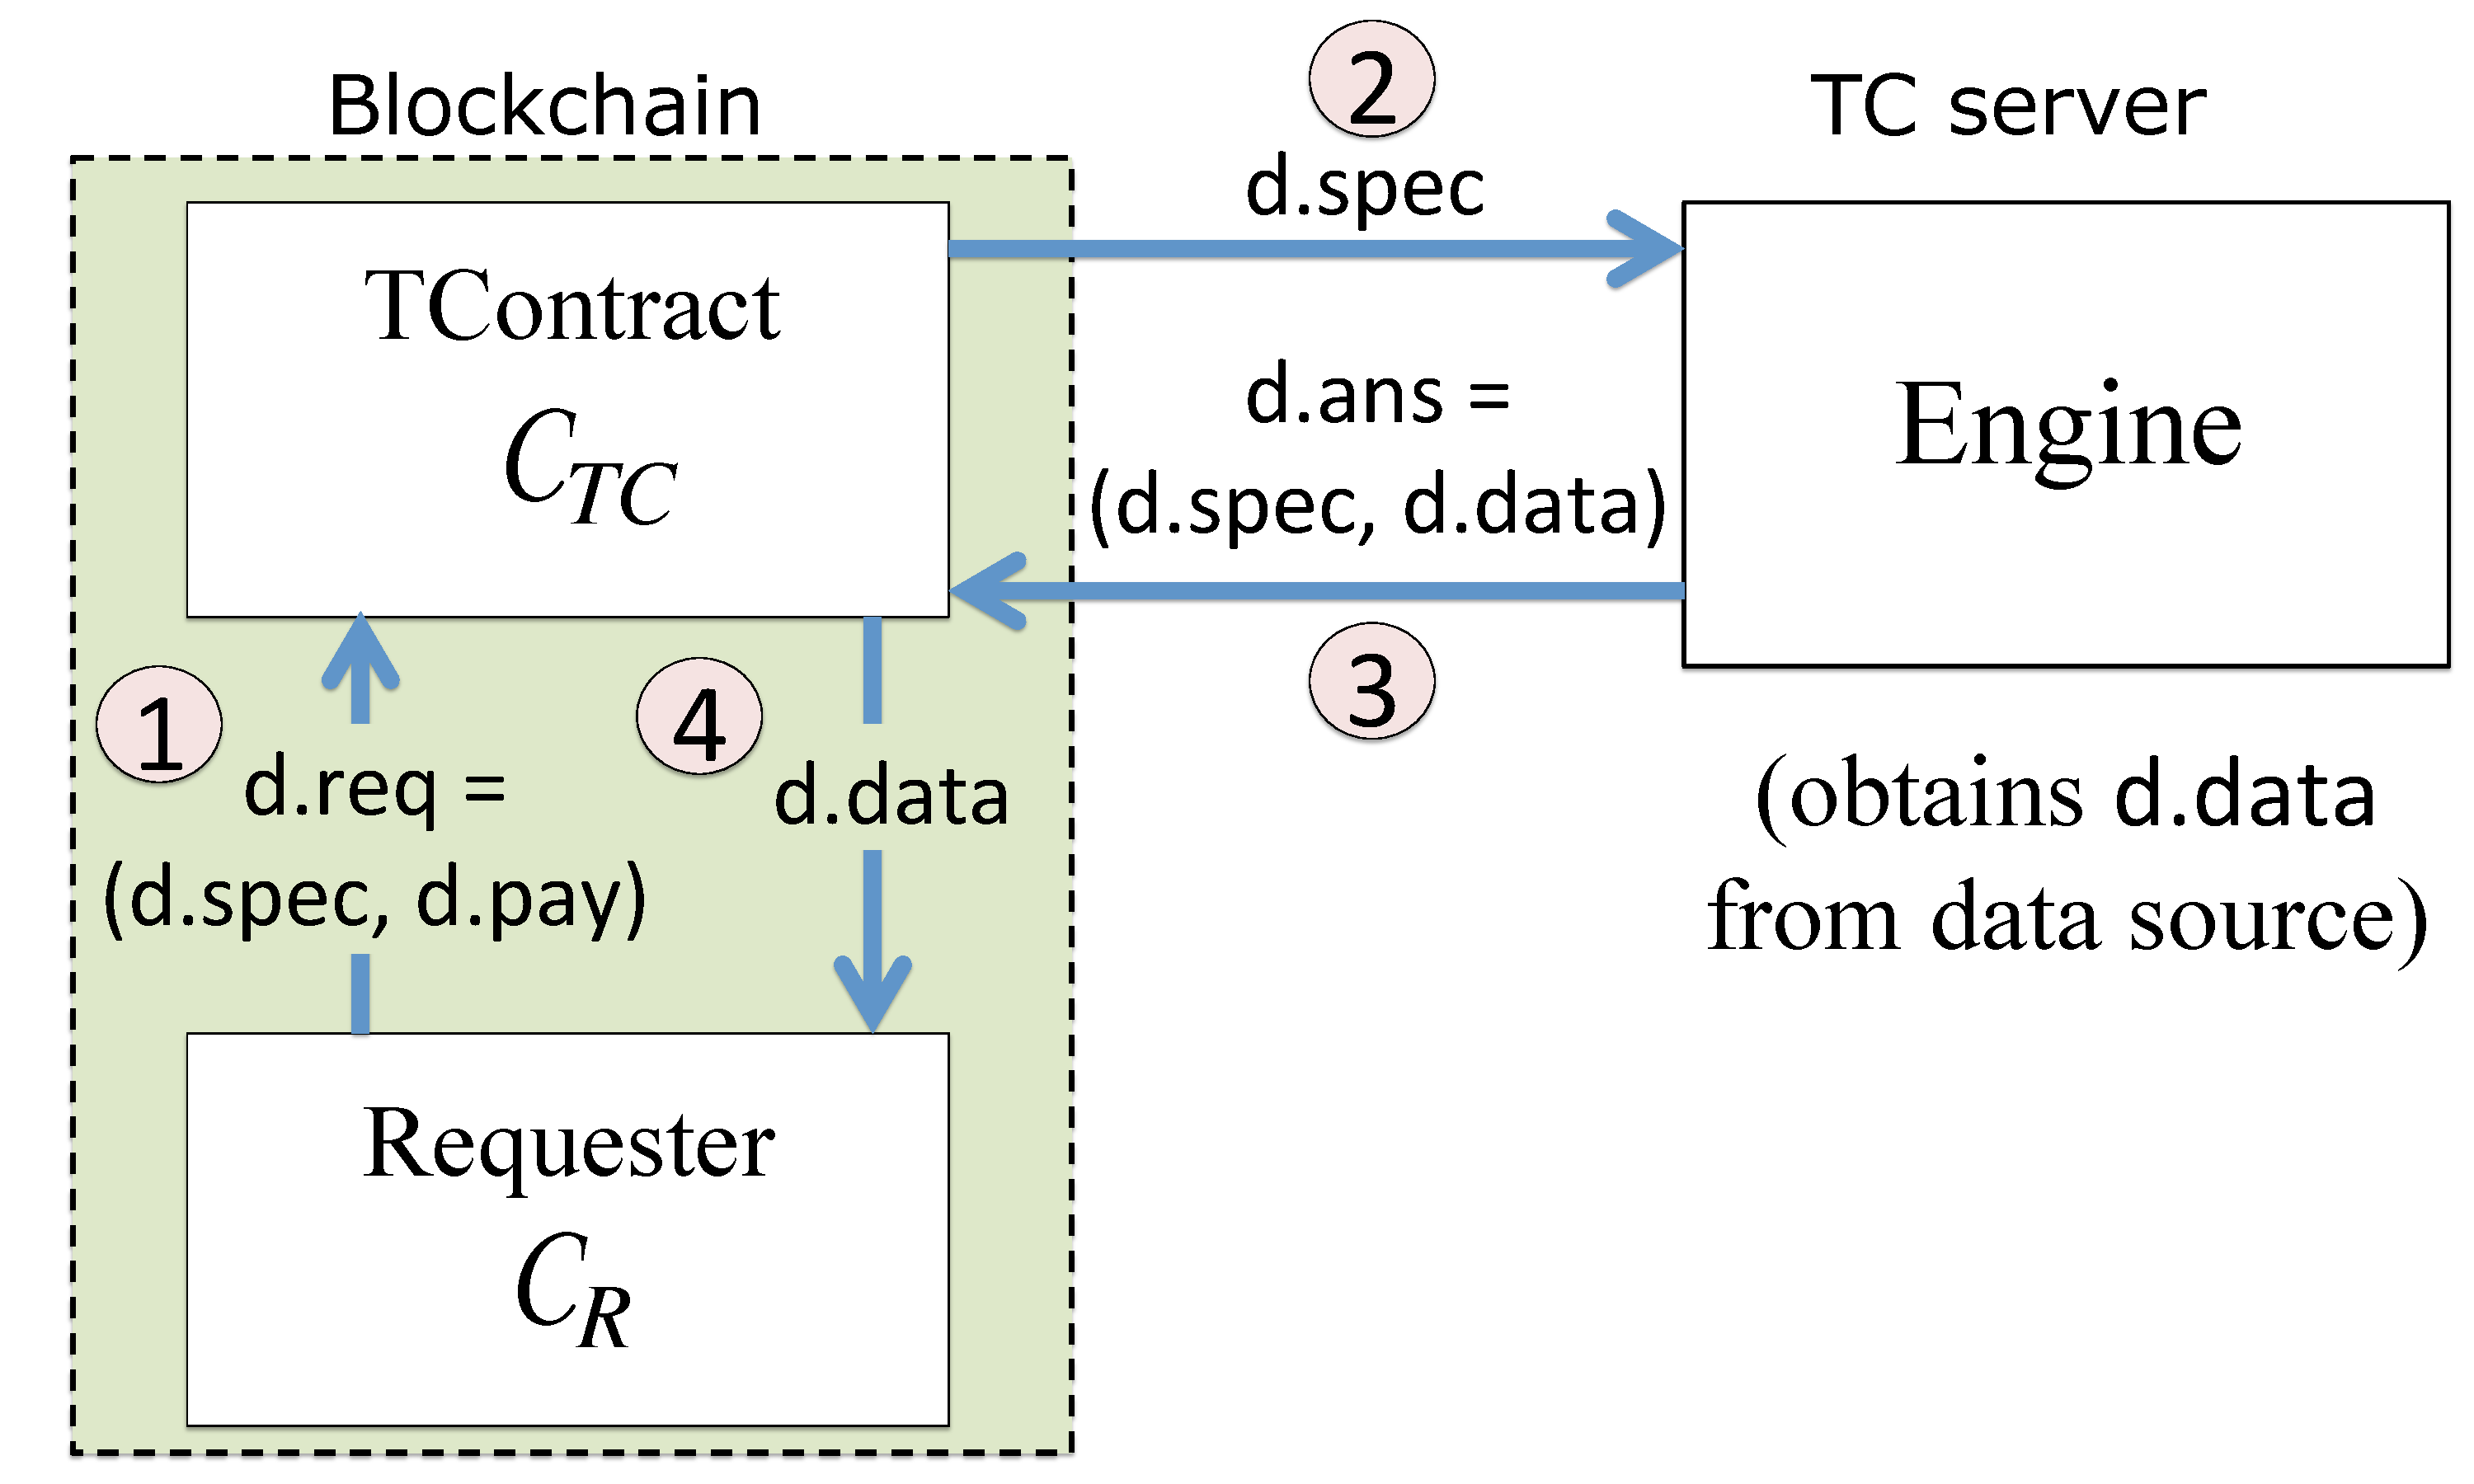
\includegraphics[width=\columnwidth]{figures/DataflowFig}
%\caption{{\bf Data flows in datagram processing.} \elaine{the figure must be changed,
%  m1 and m4 do not have id in the formal algorithm descriptions} }
%\label{fig:dataflow}
%\end{figure}


Digital signatures are needed to authenticate messages, such as $m_3$, entering the blockchain from an external source. We let $(\skTC, \pkTC)$ denote the private / public keypair associated with the \encname for such message authentication. For simplicity, Fig.~\ref{fig:dataflow} assumes that the \encname can send signed messages directly to \tcont. We explain shortly how Ethereum requires a layer of indirection such that \tc sends $m_3$ as a transaction via an Ethereum wallet \tcadd.


\subsection{Use of SGX}
\label{sec:useofsgx}

Let $\enclaveprog$ represent the code for \encname, which we presume is trusted by all system participants. Our protocols in \tc rely on the ability of SGX to attest to execution of an instance of $\enclaveprog$ and bind a public key $\pkTC$ to this instance. Here we briefly explain how we achieve these goals. First, we present a model that abstracts away implementation details in SGX, helping simplify our protocol presentation and later our security proofs. We then explain how SGX attestation is used to authenticate datagrams served by \tcont, namely through binding of $\pkTC$ to an Ethereum wallet on the blockchain. Finally, we explain how we use the clock in SGX. Our discussion draws on formalism for SGX from~\cite{sgxsok}.


%\vspace{-3mm}
\paragraph{\bf Formal model and notation.} 
We adopt a formal abstraction
of Intel SGX proposed by Shi et al.~\cite{sgxsok}. %\elaine{cite}.
Following the UC and GUC paradigms~\cite{uc,guc,juc}, Shi et al.
propose to 
abstract away the details of SGX implementation,
and instead view SGX
as a third party trusted
for both confidentiality and integrity.
Specifically, we use a global UC  
functionality $\fsgx(\sigsgx)[\enclaveprog, \relay]$
to denote (an instance of) an SGX functionality parameterized
by a (group) signature scheme $\sigsgx$.
Here $\enclaveprog$ denotes the SGX enclave program and \relay the physical
SGX host (which we assume for simplicity is the same as that for the \tc~\medname).
As described in Fig.~\ref{fig:SGX_abstraction}, upon initialization, \fsgx runs ${\sf outp} := \enclaveprog.{\bf Initialize}$()
and attests to the code of $\enclaveprog$ as well as ${\sf outp}$.
Upon a resume call with ${(\sf id, params)}$, \fsgx runs and outputs the result of
$\enclaveprog.{\bf Resume}({\sf id, params})$.
Further formalism for \fsgx is given in Appendix~\ref{sec:sgxmodel}.
%Shi et al. \elaine{cite} propose a formal
%abstraction that captures a subset of the features
%of Intel SGX. Their model follows the UC and GUC paradigm~\cite{uc,guc,juc}.
%In this paper, we use the same formal abstraction
%to model SGX (see Figure~\ref{fig:fsgx}).
%\elaine{explain more here, we can think of fsgx as a trusted third party.}

%The main idea behind the UC modeling proposed by Shi et al.
%\elaine{cite}
%
%We abstract away details of the functioning of SGX in two ways.
%First, we abstract away the use of group signatures in EPID and simply denote the keypair associated with group signatures for all legitimate SGX hosts by $(\pkM, \skM)$. 
%We let $\Sigma.{\sf Sign}({\sk}, X)$ denote a digital signature under private key $\sk$ of message $X$, and $\Sigma.{\sf Verify}({\sk}, \sigma, X)$ denote the corresponding verification operation. 
%
%Second, we model execution in SGX in terms of a functionality $\fsgx$ operating in a stateful manner on \enclaveprog \xxx[Fan]{Do we want to provide some intuition such that people with no UC background can still read our protocol correctly? For example, maybe we can briefly explain the difference between functionality and protocol?}, and specified in Figure~\ref{fig:SGX_abstraction}. $\fsgx$ may be be invoked with one of two messages to \enclaveprog : \initcall, which creates the enclave with \enclaveprog as its initial state and triggers measurement quotes, and (\resumecall, $X$) which initiates an execution of \enclaveprog on a fresh input $X$. (We assume that \enclaveprog exits only when it completes processing of a given input.) We let $\fsgx[\enclaveprog, \relay]$ denote invocation of $\fsgx$ on \enclaveprog by \relay. 
%

\begin{figure}[ht!]
\begin{boxedminipage}{\columnwidth}
\begin{center}
{\bf $\fsgx[\enclaveprog, \relay]$: abstraction for SGX}
\end{center}
\begin{tabular}{l}
{\bf{\em Hardcoded}}: $\skM$ \\[3pt]
{\bf {\em Assume}}:
{\small $\enclaveprog$ has entry points {\bf Initialize} and {\bf Resume}}\\[3pt] 

{\bf Initialize:}\\
On receive (\initcall) from $\relay$: \\
\quad Let ${\sf outp} := \enclaveprog.{\bf Initalize}()$  \\
\quad \sgray{\it //~models EPID signature.}\\
\quad $\sigatt := \sigsgx.{\sf Sign}(\skM, (\enclaveprog, {\sf outp}))$\\
\quad Output  $({\sf outp}, \sigatt)$\\[5pt]

{\bf Resume:}\\
On receive (\resumecall, {\sf id}, {\sf params}) from $\relay$: \\
\quad Let ${\sf outp} := \enclaveprog.{\bf Resume}({\sf id, params})$  \\
\quad Output ${\sf outp}$ 
\end{tabular}
\end{boxedminipage}
\caption{Formal abstraction for SGX execution capturing a subset of SGX features
sufficient for implementation of \tc.}
\label{fig:SGX_abstraction}
\label{fig:fsgx}
\end{figure}

%\vspace{-3mm}
\paragraph{Binding $\enclaveprog$ to Ethereum wallet \tcadd.}
Information can only be inserted into the blockchain in Ethereum as a transaction from a wallet.
Thus, the only way the \medname can relay messages from the \encname to \tcont is through a wallet \tcadd.
Since the \medname may corrupt messages, however, it is critical that they be authenticated by the \encname.
Since Ethereum itself already verifies signatures on transactions from externally owned accounts
(i.e., users interact with the  Ethereum blockchain through an authenticated channel),
\tc uses a trick to {\it piggyback verification of enclave signatures on top of Ethereum's already existing transaction signature verification mechanism}. 
Very simply, the \encname creates \tcadd with the public key \pkTC. 

To make this idea work fully, the public key $\pkTC$ must be hardcoded into \tcont. A client creating or relying on a contract that uses \tcont is responsible for making sure that this hardcoded $\pkTC$ has an appropriate SGX attestation before interacting with the $\tcont$  blockchain contract.  Let {\sf Verify} denote a verification algorithm for EPID signatures. Fig.~\ref{fig:att_check} gives the protocol for a client to check that \tcont is backed by a valid \encname instance. (We omit modeling here of IAS online revocation checks.)

%This protocol does not include a mechanism for \emph{revocation} of a compromised SGX instance, an issue we discuss later in the paper.

In summary, then, we may assume in our protocol specifications that {\em relying clients have verified an attestation for \encname and thus that datagram responses sent from \tcadd to \tcont are trusted to originate from \engine.} 



\begin{figure}[htb!]
\begin{boxedminipage}{\columnwidth}
\begin{center}
{\bf User: offline verification of SGX attestation}
\end{center}
\begin{tabular}{l}
{\bf {\em Inputs}}: $\pkM$, $\pkTC$, $\enclaveprog$, $\sigatt$ \\[5pt]
{\bf Verify:} \\
Assert $\enclaveprog$ is the expected enclave code\\
Assert $\sigsgx.{\sf Verify}(\pkM, \sigatt, (\enclaveprog, \pkTC))$ \\
Assert \tcont is correct and parametrized w/ \pkTC\\
\sgray{\it //~now okay to rely on \tcont}
\end{tabular}
\end{boxedminipage}
\caption{A client checks an SGX attestation on the enclave's code $\enclaveprog$ and public key $\pkTC$.
  The client also checks that $\pkTC$ is hardcoded into \tc blockchain contract \tcont before using \tcont.
} 
\label{fig:att_check}
\end{figure}


%\vspace{-3mm}
\paragraph{\bf SGX Clock.}
As noted above, the trusted clock for SGX provides only relative time with respect to a reference point.
To work around this, the \encname is initialized with the current wall-clock time provided by a trusted source, e.g., the \medname (under a trust-on-first-use model).
In the current implementation of \tc, clients may, in real time, request and verify a fresh timestamp---signed by the \encname under \pkTC---via a web interface in the \medname.
Thus, a client can determine the absolute clock time of the \encname to a degree of accuracy bounded by the round-trip time of its attestation request plus the attestation verification time---hundreds of milliseconds in a wide-area network.
This high degree of accuracy is potentially useful for some applications but only loose accuracy is required for most. Ethereum targets a block interval of 12 s and the clock serves in \tc primarily to: (1) Schedule connections to data sources and (2) To check TLS certificates for expiration when establishing HTTPS connections. For simplicity, we assume in our protocol specifications that the \encname clock provides accurate wall-clock time in the canonical format of seconds since the Unix epoch January 1, 1970 00:00 UTC.

We let $\clock()$ denote measurement of the SGX clock from within the enclave, expressed as the current absolute (wall-clock) time. 



\subsection{Shrinking the TCB}
\label{sec:shrinking-tcb}

As described in Section~\ref{sec:architecture}, \tc has two trusted components: the \encname and \tcont.
These components must communicate with each other, but can only do so over insecure channels (through the \medname).
Moreover, these components comprise very different properties.
\tcont resides on the blockchain where users can interact directly with \tc and all computation is verifiable, expensive, and transparent.
The \encname provides a private and less expensive environment, but all interaction (user or otherwise) must go through an untrusted intermediary.

The simplest way to ensure authentic communication between the components is to have both perform verification;
\tcont receives signed messages from the \encname and verifies the signatures,
and the \encname receives raw blocks and verifies that they are well-formed.
Unfortunately, both of these verification mechanisms require a large amount of computation and complex code.

We describe above how we bind the \encname to an Ethereum wallet, which removes the need to do explicit signature verification in \tcont (which would be extremely expensive).
In order to reduce the cost of this verification inside the \encname, we leverage the fact that all messages from the \encname to \tcont are responses to existing requests.
Instead of verifying the request parameters in the \encname, we can verify in \tcont that the \encname is responding to the correct request.
For each request, \tcont stores the parameters of that request and the \encname includes the parameters it used to fulfill a request in its response.
This allows \tcont to check that the parameters match and simply reject the response if they do not.
Because storing parameters and checking equality are extremely simple, this removes a complex verification step from the TCB.

While this may appear to open some attack (e.g., the \medname can send bogus requests and the \encname will attempt to respond),
all of these attacks amount to DoS attacks from the network or the \medname---attacks to which we were already susceptible.

We note that this technique is actually quite general.
Given any system with two trusted components communicating over an insecure channel, if one component only response to requests from the other,
the requesting component can store parameters and the responding component can include them in a response.
This allows the responding component to omit integrity verification on its incoming requests without compromising the integrity of the system as a whole.



\subsection{A Payment-Free Basic Protocol}
\label{sec:payment-free-protocol}

For simplicity, we first specify a payment-free version of our basic protocol, i.e.~one that does not include gas or fees. Later, in our implementation discussion, we explain how we handle these two resources and we prove payment-related properties in the paper appendix. For simplicity, we assume a single instance of \engine, although our architecture could scale up to multiple enclaves and even server instances. To show messages corresponding to those in Fig.~\ref{fig:dataflow}, we use the label $(\msgi{i})$.

%\vspace{-3mm}
\paragraph{The Requester Contract $\reqcont$.}
The requester contract $\reqcont$ sends a request of the form $(\dgform, \dgcallback)$ to the \tcontract \tcont.

%\vspace{-3mm}
\paragraph{The \tcontract \tcont.} 
The \tcontract accepts a datagram request from \reqcont, assigns it a unique ${\sf id}$, and records the request.
Our \tcs\ \medname\ \relay monitors requests received by \tcont and forwards them to an SGX enclave.
When $\tcont$ obtains a valid response from $\tcadd$, it sends the resulting datagram $\dgm$ to the entry point \dgcallback specified by the requesting contract \reqcont.
As explained in Section~\ref{sec:shrinking-tcb}, \tcont must check that the response comes from \tcadd and that $\dgform' = \dgform$ to ensure validity.
The first is sufficient to prove that the response was produced by \engine, while the second ensures that \relay cannot corrupt requests despite \engine not performing explicit validation.
\tcont is specified in Fig.~\ref{fig:tc-contract}. Here, Call denotes a call to a contact entry point. 

\begin{figure}[!htb]
\begin{tabularx}{\linewidth}{|@{\hspace{3pt}}r@{\hspace{1ex}}X@{\hspace{3pt}}|}
  \hline

  \multicolumn{2}{|c|}{{\bf Program for Town Crier blockchain contract \tcont}} \\ [1ex]

  {\bf Initialize:} &  Counter := 0 \\[1ex]

  {\bf Request:} & On recv $(\dgform, \dgcallback)$ from some $\reqcont$: \\
                 & \dgid :=  Counter; \ \ Counter := Counter + 1 \\
                 & Record $(\dgid, \dgform, \dgcallback)$ \hfill \sgray{\it //~\msgi{1}} \\[1ex]

  {\bf Deliver:} & On recv $(\dgid, \dgform, \dgm)$ from $\tcadd$: \\
                 & Retrieve recorded $(\dgid, \dgform', \dgcallback)$ \\
                 & Assert $\dgform = \dgform'$ \\
                 & Call ${\dgcallback}({\dgm})$ \hfill \sgray{\it //~\msgi{4}} \\

  \hline
\end{tabularx}
\caption{
The Town Crier \tcontract \tcont.
}
\label{fig:tc-contract}
\end{figure}

%\vspace{-3mm}
\paragraph{The \encname \engine.} When initialized through {\bf Initialize}(), \engine ingests the current wall-clock time; by storing this time and setting a clock reference point, it calibrates its absolute clock. It generates an ECDSA keypair $(\pkTC,\skTC)$ (parameterized as in Ethereum), where $\pkTC$ is bound to the \engine instance through insertion into attestations.  

Upon a call to {\bf Resume}$({\sf id}, {\sf params})$, \engine contacts the data source specified by {\sf params} via HTTPS and checks that the corresponding certificate {\sf cert} is valid. (We discuss certificate checking in Appendix~\ref{sec:impl}.) Then \engine fetches the requested datagram and returns it to \relay along with $\dgform$ and $\dgid$, all digitally signed with $\skTC$.  Fig.~\ref{fig:engineprotocol} shows the protocol for \engine.

\begin{figure}[!h]
\begin{boxedminipage}{\columnwidth}
\begin{center}
{\bf Program for \tcs~\encname ($\enclaveprog$)}
\end{center}
\begin{tabular}{l} 
{\bf Initialize}\,$({\sf void})$ \\ %{\it //~called only once upfront}\\
%\quad Set clock reference point\\
%\quad Record $T_0$ \elaine{this is never used} \\ 
%\elaine{i deleted the clock implementation, we can separate abstraction from implementation.}\\
\quad \sgray{\it// Subroutine call from $\fsgx$, which attests to}\\ 
\quad \sgray{\it// $\enclaveprog$ and $\pkTC$. See Figure~\ref{fig:SGX_abstraction}.} \\
\quad $(\pkTC, \skTC) := \Sigma.{\sf KeyGen}(1^\lambda)$\\
%\quad Record $(\pkTC, \skTC)$\\
\quad Output $\pkTC$   \\[3pt]

%{\bf Attest}:  On recv \attcall: \\ %{\it //~called only once upfront}\\
%\quad $T := \clock()$\\
%\quad Call quoting enclave with supp.~data $(\pkTC, T)$
%\\[5pt]

{\bf Resume}\,$(\dgid, \dgform)$\\
\quad Parse ${\sf params}$ as $(\weburl, \dgspec, T) $:\\
\quad Assert $\clock() \geq T.{\sf min}$\\
\quad Contact $\weburl$ via HTTPS, obtaining ${\sf cert}$ \\
\quad Verify {\sf cert} is valid for time $\clock()$\\
\quad Obtain webpage $w$ from $\weburl$ \\
\quad Assert $\clock() \leq T.{\sf max}$\\
\quad Parse $w$ to extract \dgm with specification \dgspec \\
\quad $\sigma := \Sigma.{\sf Sign}({\skTC}, ({\sf id}, {\sf params}, {\sf data}))$\\
\quad Output $(({\sf id}, {\sf params}, {\sf data}), \sigma)$
\end{tabular}
\end{boxedminipage}
\caption{
The \tcs~\encname \engine.
} 
\label{fig:engineprotocol}
\end{figure}

%\vspace{-3mm}
\paragraph{The \medname \relay.}
As noted in Section~\ref{sec:architecture},
\relay bridges the gap between the \encname and the blockchain in three ways.
(1) It scrapes the blockchain and monitors \tcont for new requests $(\dgid, \dgform)$.
(2) It boots the \encname with \engine.{\bf Initialize}() and calls \engine.{\bf Resume}$(\dgid, \dgform)$ on incoming requests.
(3) it forwards datagrams from \engine to the blockchain.
Recall that it forwards already-signed transacations to the blockchain as \tcadd.
%Recall that it sends transactions to the blockchain and thus forwards responses as \tcadd.
The program for \relay is shown in Fig.~\ref{fig:relayprotocol}.
The function {\sf AuthSend} inserts a transaction to blockchain (``as $\tcadd$'' means the transaction is already signed with $\skTC$).
An honest \medname will invoke \engine.{\bf Resume} exactly once with the parameters of each valid request and never otherwise.

\begin{figure}[h!]
\begin{tabularx}{\linewidth}{|@{\hspace{3pt}}p{1em}@{\hspace{1ex}}X@{\hspace{3pt}}|}
  \hline

  \multicolumn{2}{|c|}{\bf Program for Town Crier \medname $\relay$} \\[1ex]

  \multicolumn{2}{|l|}{\bf Initialize:} \\
                    & Send \initcall to $\fsgx[\enclaveprog, \relay]$ \\
                    & On recv $(\pkTC, \sigatt)$ from $\fsgx[\enclaveprog, \relay]$: \\
                    & \quad Publish $(\pkTC, \sigatt)$ \\[1ex]

  \multicolumn{2}{|l|}{{\bf Handle}$(\dgid, \dgform)$:} \\
                    & Parse \dgform as $(\_, \_, T)$ \\
                    & Wait until ${\sf clock}() \geq T.{\sf min}$ \\
                    & Send $(\text{\resumecall}, \dgid, \dgform)$ to $\fsgx[\enclaveprog, \relay]$ \\
                    & On recv $((\dgid, \dgform, \dgm), \sigma)$ from \\ & $\fsgx[\enclaveprog, \relay]$: \\
                    & \quad  {\sf AuthSend} $(\dgid, \dgform, \dgm)$ to \tcont as \tcadd \\
                    & \quad \sgray{\it //~send out $\msgi{3}$} \\[1ex]

  \multicolumn{2}{|l|}{\bf Main:} \\
                    & Loop Forever: \\
                    & \quad Wait for \tcont to records request $(\dgid, \dgform, \_)$: \\
                    & \quad Fork a process of {\bf Handle}$(\dgid, \dgform)$ \\
                    & End \\

  \hline
\end{tabularx}
\caption{The Town Crier \medname \relay.}
\label{fig:relayprotocol}
\end{figure}




\section{\tc Implementation Details}
\label{sec:impl}

We now present further, system-level details on the \tc contract \tcont and the two parts of the \tc server, the \encname and \medname.

\subsection{TC Contract} 

We implement \tcont with fees as described in Section~\ref{sec:gas-protocol} in Solidity,
a high-level language with JavaScript-like syntax which compiles to Ethereum Virtual Machine bytecode---the language Ethereum contracts use.

In order to handle the most general type of requests---including encrypted parameters---the \tcont implementation requires two parameter fields:
a single byte specifying the type of request (e.g.~flight status) and a byte array of user-specified size.
This byte array is parsed and interpreted inside the \encname, but is treated as an opaque byte array by \tcont.
For convenience, we include the timestamp of the current block as an implicit parameter.

To guard against the \medname tampering with request parameters, the \tcont protocol includes $\dgform$ as an argument to {\bf Deliver} which validates against stored values.
To reduce this cost for large arrays, we store and verify $\text{SHA3-256}({\sf typeByte} || {\sf timestamp} || {\sf paramArray})$.
The \medname scrapes the raw values for the \encname which computes the hash and includes it as an argument to {\bf Deliver}.



\subsection{TC Server}
Using the recently released Intel SGX SDK~\cite{sgxsdk}, we implmented the \tc
Server as an SGX-enabled application in C++. In the programming model supported
by the SGX SDK, the body of an SGX-enabled application runs as an ordinary
user-space application, while a relatively small piece of security-sensitive
code runs in the isolated environment of the SGX enclave.

The enclave portion of an SGX-enabled application may be viewed as a shared
library exposing an API in the form of \emph{ecalls} to be invoked by the
untrusted application. Invocation of an ecall transfers control to the enclave;
the enclave code runs until it either terminates and explicitly releases
control, or some special event (e.g., exception) happens~\cite{sgxmanual}.
Again, as we assume SGX provides ideal isolation, the untrusted application
cannot observe or alter the execution of ecalls.

Enclave programs can make \emph{ocalls} to invoke functions defined outside of
the enclave. An ocall triggers an exit from the enclave; control is returned
once the ocall completes. As ocalls execute outside the enclave, they must be
treated by enclave code as untrusted. 


\begin{figure}[h]
    \centering
%    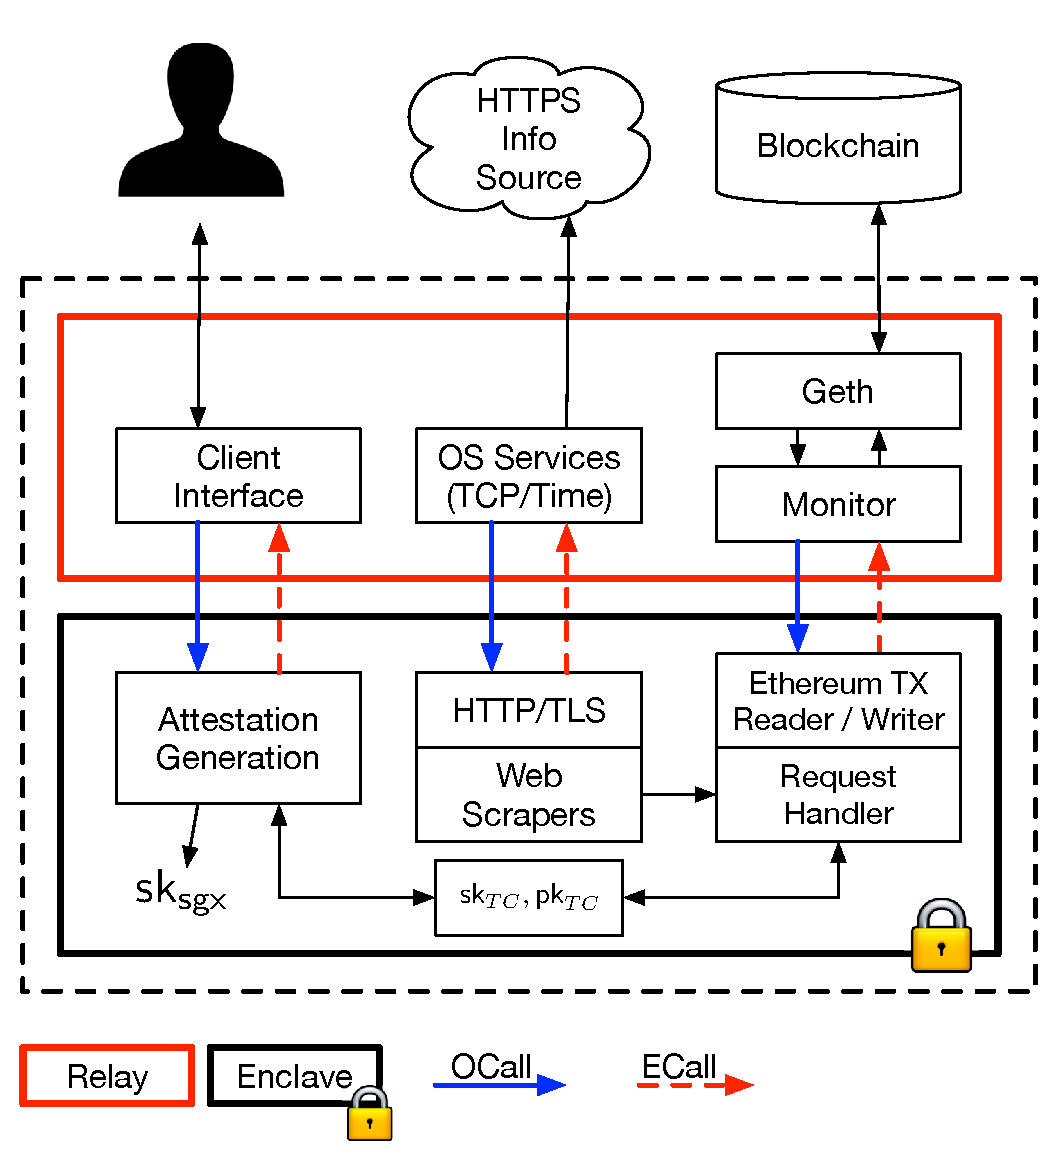
\includegraphics[width=0.45\textwidth]{figures/impl}

\begin{tikzpicture}
  [box/.style={entity, text width=1.5cm, inner sep=5pt},
   untrusted/.style={fill=red!33},
   double/.style={rectangle split, rectangle split parts=2},
   ecall/.style={color=blue,thick},
   ocall/.style={color=red!80!black,thick}]
  \matrix (m) [row sep=1.2em, column sep=0.6em]{
    \node[inner sep=0pt,anchor=south] (user) {
\includegraphics[width=1cm]{figures/user}}; &
    \node[inner sep=0pt,draw,cloud,aspect=2.0,align=center,anchor=south](cloud) {\footnotesize HTTPS \\ websites}; &
    \node[box, cylinder, shape border rotate=90, aspect=.2,anchor=south](bc){blockchain};  \\[0.9em]

    \node[box,fill=white] (client) {Client \\ Interface}; & 
    \node[box,fill=white] (net) {TCP}; & 
    \node[box,fill=white,double,text width=2cm] (monitor) {\texttt{geth} \nodepart{second}{Blockchain \\ Interface}}; \\[0.6em]

    \node[box] (att) {Attestation \\ Generation}; &
    \node[box,double] (https) {HTTPS \nodepart{second}{Web \\ Scrapers}}; &
    \node[box,double,text width=2cm,] (req h){Ethereum TX \\ Reader/Writer \nodepart{second}{Request Handler}}; \\

    & \node[box,text width=2cm] (keys) {\pkTC, \skTC}; & \\
  };
  \node[anchor=west] (sk) at (keys.west-|att.west) {\skM};

  \draw[<->,thick] (user) -- (client);
  \draw[<->,thick] (net) -- (cloud);
  \draw[<->,thick] (monitor) -- (bc);

  \draw[->,ocall,transform canvas={xshift=-2mm}] (https) to (net);
  \draw[->,ocall,dashed,transform canvas={xshift=+2mm}] (net) to (https);

  \draw[->,ecall,transform canvas={xshift=-2mm}] (client) -- (att);
  \draw[<-,ecall,dashed,transform canvas={xshift=+2mm}] (client) -- (att);

  \draw[->,ecall,transform canvas={xshift=-2mm}] (monitor) -- (req h);
  \draw[<-,ecall,dashed,transform canvas={xshift=+2mm}] (monitor) -- (req h);

  \draw[<->,thick] (https.two east) -- (https.two east -| req h.two west);

  \draw[->,thick] (req h.south) |- (keys.east);
  \draw[->,thick] ([xshift=1.25em]att.south)  |- (keys.west);
  \draw[->,thick] (att.south-|sk.north) -- (sk);

  \begin{pgfonlayer}{background}
    \node [bg-box, inner sep=1.2em, tc-server-color, fit=(client)(monitor)(keys)] {};
    \node [inner sep=0.6em, untrusted, fit=(client) (net) (monitor)] {};
    \node [inner sep=0.6em, trusted, fit=(att) (https) (req h) (keys)] {};
  \end{pgfonlayer}

    \matrix (legend) [below=1.2em of m, matrix of nodes, column sep=0.75em, align=center]
  {
    \node[inner xsep=0] {\small \bf Legend:}; &
    \node[untrusted] (relay-leg) {\small Relay\vphantom{Ry}}; &
    \node[trusted] (enc-leg) {\small Enclave\vphantom{Ry}}; &
    \node[tc-server-color,rounded corners,text width=2.5em] (server-leg) {\small Server\vphantom{Ry}}; &
    \node[text width=1.75em] (ecall-leg) {}; &
    \node[text width=1.75em] (ocall-leg) {}; \\
  };

  \path[->,ecall,above] (ecall-leg.west) edge node {\small ecall} (ecall-leg.east);
  \path[<-,ecall,dashed,transform canvas={yshift=-0.4em}] (ecall-leg.west) edge (ecall-leg.east);

  \path[->,ocall,above] (ocall-leg.west) edge node {\small ocall} (ocall-leg.east);
  \path[<-,ocall,dashed,transform canvas={yshift=-0.4em}] (ocall-leg.west) edge (ocall-leg.east);
\end{tikzpicture}
\caption{Components of \tc Server}
\label{fig:tcserver_impl}
\end{figure}

For \tc, we recall that Fig.~\ref{fig:engineprotocol} shows the \encname code
$\engine$. Fig.~\ref{fig:relayprotocol} specifies the operation of the \medname,
the untrusted code in \tc, which we emphasize again provides essentially only
network functionality. We now give details on the services in the \encname and
the \medname and describe their interaction, as summarized in
Fig.~\ref{fig:tcserver_impl}.

\paragraph{\bf The \encname.} There are three components to the enclave code
\engine: An HTTPS service, Web Scrapers, which interact with data sources, and a
Request Handler, which services datagram requests. 

\vspace{2mm}

\noindent\emph{HTTPS Service.} We recall that the enclave does not have direct
access to host network functionality. \tc thus partitions HTTPS into a trusted
layer, consisting of HTTP and TLS code, and an untrusted layer that provides
low-layer network service, specifically TCP.  This arrangement allows the
enclave to establish a secure channel with a web server: The enclave itself
performs the TLS handshake with a target server and performs all cryptographic
operations internally, while the untrusted process acts as a network interface
only. We ported a TLS library (mbedTLS) into the SGX environment, as well as
HTTP code, which we minimized to meet the web-scraping requirements of \tc while
keeping the TCB small. To verify certificates presented by remote servers, we
hardcoded a collection of root CA certificates into the enclave code; in the
first version of \tc, the root CAs are identical to those in Chrome~\cite{}. By using its internal, trusted wall-clock time, it is possible to verify that a certificate has not expired. (We briefly discuss revocation in Appendix~\ref{sec:future}.)

\vspace{2mm}

\noindent\emph{Web Scrapers.} We implemented scrapers for our examples in Section~\ref{sec:applications} in an ad hoc manner for our initial implementation of \tc, and defer more principled, robust approaches to future work. 

\vspace{2mm}

\noindent\emph{Request Handler.} The Request Handler has two jobs: (1) Ingesting
a datagram request by parsing it in the serialization format specified by
Ethereum, decrypting it (if it's a private-datagram request), and dispatching
its parameters to the right scraper; and (2) Returning the response to the
request by generating an Ethereum transaction containing the requested datagram
(and parameters), serializing it as a blockchain transaction, and signing it
using \skTC. We implemented the Ethereum ABI and RLP, which respectively specify
the serialization of arguments and transactions in Ethereum. 

\vspace{2mm}

\noindent\emph{Attestation Generation.} Recall in Section \ref{sec:background}
we mentioned that an \emph{attestation} is an \emph{report} digitally signed by
the Intel-provided Quoting Enclave (QE).  Therefore two phases are involved in
generating \att. First, the \encname calls \texttt{sgx\_create\_report} to
generate a report with QE as the target enclave. Then the \medname forwards the
report to QE and calls \texttt{sgx\_get\_quote} to get a signed version of the
report, namely an attestation.

\paragraph{The \medname.} The \medname encompasses three components: A Client Interface, which serves attestations and timestamps, OS services, including networking and time services, and a Blockchain Interface. 

\vspace{2mm}

\noindent\emph{Client Interface.} As described in Section \ref{sec:architecture},
a client starts using \tc by requesting and verifying an attestation \att and checking the correctness of the clock in the \tc enclave using a fresh timestamp.
The Client Interface caches \att upon initialization of \engine. When it receives a web request from a client for an attestation,
it issues an ecall to the enclave to obtain a
Unix timestamp signed using \skTC, which it returns to the client along with \att. The client verify \att 
using the Intel Attestation Service (IAS)~\cite{} and then verify the timestamp using $\pkTC$ and check it using any trustworthy time service. 

\vspace{2mm}

\noindent\emph{OS services.} The \encname relies on the \medname to access networking and 
wall-clock time provided by the OS and implemented as ocalls.

\vspace{2mm}

\noindent\emph{Blockchain Interface.} The \medname's Blockchain Interface monitors the
blockchain for incoming requests and places transactions on the blockchain in order to
deliver datagrams. The Blockchain Interface incorporates an 
official Ethereum client, Geth~\cite{geth}. This Geth client can be configured with a JSON RPC server.  
The \medname  communicates with the blockchain indirectly via RPC calls to this server. For example, to insert a signed transaction, the \medname simply calls
\texttt{eth\_sendRawTransaction} with the byte array of the serialized
transaction. We emphasize that as the enclave holds \skTC, transactions are signed within the enclave.


\section{Extensions}

\subsection{Handling Transaction Fees}

To mitigate potential Denial-of-Service (DoS) attacks, 
Ethereum employs a fee mechanism, referred to as ``gas'', 
where the submitter of a transaction (that invokes
an entry point in the contract) pays a  
transaction fee
roughly proportional to the execution time of the 
corresponding entry point.

\paragraph{Notations and assumed execution model.}
In Figure \elaine{fill}, we
use the notation $\sbrown{\Delta F}$
to denote transaction fees (i.e., gas), 
where $\Delta$ is a type annotation 
and ${\tt F}$ denotes the numerical amount of the  
gas. Other non-gas, normal currency units 
are denoted as $\smaroon{\$ F}$ where $\$$ is a type annotation,
and ${\tt F}$ denotes the amount of the currency. 
For simplicity, our notational system assumes 
that gas and normal currency adopt
the same currency unit. 

We assume that the blockchain contract adopts the following execution model
for gas which closely resembles Ethereum's execution model:
\begin{itemize}[leftmargin=5mm]
\item
{\it Providing gas.} 
When a transaction is submitted, it invokes an entry point in the contract.
The transaction submitter provides a gas amount to activate the entry point. 
\item
{\it Extra gas.} 
If extra gas remains at the end of the execution (after invoking an entry point),
all extra gas is refunded to the transaction submitter at the end.
\item
{\it Gas exhaustion.} 
Gas exhaustion is dealt with in the following manner.
Consider each entry point of the contract as a function. 
Functions can call other functions.
Each function can specify a gas upper bound not to exceed
the remaining gas of the parent function (and if left unspecified,
the upper bound is implicitly set to all remaining gas of the parent function).
If execution of the function exhausted the per-function gas 
upper bound, the function execution is aborted and 
state reverted to before the function is invoked.
\end{itemize}

\begin{figure}
\begin{tabularx}{\linewidth}{|@{\hspace{3pt}}r@{\hspace{1ex}}X@{\hspace{3pt}}|}
  \hline

  \multicolumn{2}{|c|}{{\bf Town Crier blockchain contract \tcont with fees}} \\ [1ex]
  {\bf Request:} & On recv $({\sf id}, {\sf params}, 
{\sf callback},  
{\color{blue} \Time_{\text{timeout}}},
\sbrown{\Delta F_{\text{request}}}$ $+$ 
$\smaroon{\$F_{\text{deliver}}})$ from some $\reqcont$: \\
		& Assert ${\color{blue} \Time_{\text{timeout}}} > {\sf cur\_time}$\\
                 & Record $({\sf id}, {\sf params}, {\sf callback}, \smaroon{\$ F_{\text{deliver}}}, {\color{blue} \Time_{\text{timeout}}}, {\reqcont})$
%\elaine{this makes it look like it's sending money}
\\[-10pt]
    & {\it {\color{gray} {//~at most ${{\Delta F_{\textrm{request}}}}$ {gas consumed}}} }\\[-10pt]
    & {\it {\color{gray} {//~all remaining {gas returned to $\reqcont$}}} }\\[-10pt]
    & {\it {\color{gray} {//~$\smaroon{\$ F_{\text{deliver}}}$} held by contract}} \\
  {\bf Deliver:} & On recv $({\sf id}, {\sf params}, {\sf data}, 
$\sbrown{\Delta {\tt F_{\text{deliver}}}}$ )$ from $\tcadd$: \\
                 & Let $({\sf id}, {\sf params'}, {\sf callback}, \smaroon{\$ F'_{\text{deliver}}}, {\color{blue} \Time_{\text{timeout}}}, \_)$ be the first recorded tuple for ${\sf id}$\\
 & Assert ${\color{blue} \Time_{\text{timeout}}} > {\sf cur\_time}$ \\
                 & Assert ${\sf params} = {\sf params}'$\\
                &   Assert $\smaroon{\$ F'_{\text{deliver}}} \leq \sbrown{\Delta F_{\text{deliver}}}$\\
		& Set ${\sf bDelivered}[{\sf id}]$ \\
                 & Send $\smaroon{\$F'_{\text{deliver}}}$ to $\tcadd$ \\
                 & Call ${\sf callback}({\sf data})$ \\[-10pt]
    & {\it {\color{gray} {//~at most ${{\Delta F_{\textrm{deliver}}}}$ {gas consumed}}} }\\[-10pt]
    & {\it {\color{gray} {//~all remaining {gas returned to $\tcadd$}}} }\\

{\bf Cancel:} & On recv $({\sf id}, \sbrown{\Delta F_{\text{cancel}}})$ 
from some $\reqcont$\\
  & Let $({\sf id}, \_, \_, \smaroon{\$ F_{\text{deliver}}}, {\color{blue} \Time_{\text{timeout}}}, \reqcont')$ be the first recorded tuple for ${\sf id}$ \\
   & Assert $\reqcont = \reqcont'$\\
   & Assert ${\sf bDelivered}[{\sf id}]$ not set \\ 
   & Assert ${\sf cur\_time} \geq {\color{blue} \Time_{\text{timeout}}}$\\
  & Send $\smaroon{\$ F_{\text{deliver}}}$ to \reqcont\\
  \hline
\end{tabularx}
\caption{
Town Crier contract \tcont reflecting fees.
$\sbrown{\Delta F_{\text{request}}}$ denotes the gas for executing the {\bf Request} 
entry point. 
$\sbrown{\Delta F_{\text{deliver}}}$ denotes the gas for executing the {\bf Deliver} entry point
that includes the user-defined ${\sf callback}$.
\smaroon{\$F_{\text{deliver}}} denotes 
${\tt F_{\text{deliver}}}$ amount of 
explicit, non-gas currency units.
Essentially, the requester first pays 
$\smaroon{\$ F_{\text{deliver}}}$ currency units which will be used to refund
the $\sbrown{\Delta F_{\text{deliver}}}$ amount of gas
that $\pksgx$ will need to put in to call the {\bf Deliver} entry point.
}
\label{tbl:tc-contract}
\end{figure}

\begin{figure}[!h]
\begin{boxedminipage}{\columnwidth}
\begin{center}
{\bf Program for Town Crier \medname $\relay$}
\end{center}
\begin{tabular}{l}
{\bf Initialize}: Same as Figure~\ref{fig:relayprot}\\
%Send \initcall to $\fsgx[\enclaveprog, \relay]$\\
%On recv $(\pkTC, \sigatt)$ from $\fsgx[\enclaveprog, \relay]$:\\
%\quad Publish $(\pkTC, \sigatt)$\\[5pt]

{\bf  Loop forever}: \\
Whenever \tcont receives 
a request
$({\sf id}, {\sf params}, \_, \_,$ $\sbrown{\Delta F_{\text{request}}}$ $+ \smaroon{\$ F_{\text{deliver}}})$:  \\  %\sgray{{\it //~{\bf msg.}~$m_2$}}\\
\ \quad Assert $\sbrown{\Delta F_{\text{min}}} \leq  
\smaroon{\$ F_{\text{deliver}}}
\leq \sbrown{\Delta F_{\text{max}}} $ \\
\ \quad Send $(\text{\resumecall}, ({\sf id}, {\sf params}, {\tt F_{\text{deliver}}} )$ to $\fsgx[\enclaveprog, \relay]$ \\
\ \quad On recv $(({\sf id}, {\sf params}, {\sf data}), \sigma)$ from $\fsgx[\enclaveprog, \relay]$:\\ 
\ \quad \quad  
{\sf AuthSend} $(({\sf id}, {\sf params}, {\sf data}, \sbrown{\Delta F_{\text{deliver}}}))$ to \tcont as \tcadd \\
\hspace{50mm} \sgray{\it //~{\bf msg.}~$m_3$}
\end{tabular}
\end{boxedminipage}
\caption{The Town Crier \medname \relay (with fees).}
\label{fig:relayprot}
\end{figure}

\begin{figure}[!h]
\begin{boxedminipage}{\columnwidth}
\begin{center}
{\bf Program for \tcs~\encname ($\enclaveprog$)}
\end{center}
\begin{tabular}{l}
%{\bf Inputs}:  ${\sf params}$, \\[5pt]
%{\bf Initialize}:  On recv (\initcall, $T_0)$: \\ %{\it //~called only once upfront}\\
{\bf Initialize}:  
Same as Figure \elaine{refer}
\\[3pt]

%{\bf Attest}:  On recv \attcall: \\ %{\it //~called only once upfront}\\
%\quad $T := \clock()$\\
%\quad Call quoting enclave with supp.~data $(\pkTC, T)$
%\\[5pt]

{\bf Resume:} On recv (\resumecall, $({\sf id}, {\sf params}, {\tt F_{\text{deliver}}}))$\\
\quad Same as before except the last two statements:\\
\quad $\sigma := \Sigma.{\sf Sign}({\skTC}, ({\sf id}, {\sf params}, {\sf data},
\sbrown{\Delta F_{\text{deliver}}}))$\\
\quad Output $(({\sf id}, {\sf params}, {\sf data}, \sbrown{\Delta F_{\text{deliver}}}), \sigma)$
\end{tabular}
\end{boxedminipage}
\caption{
The \tcs~\encname \engine.
} 
\label{fig:engineprot}
\end{figure}



\paragraph{Town Crier protocol with transaction fees.}
Our basic Town Crier implements a policy where the requester pays for all gas 
needed and Town Crier in effect pays nothing.
We now describe how this can be realized by modifying
the fee-free protocol described in Section \elaine{refer}. 

\elaine{need to add time to all the description below.}
\begin{itemize}[leftmargin=5mm]
\item
{\it Initialization.}
To initialize the system, we assume that Town Crier 
deposits a fixed amount $\sbrown{\Delta F_{\text{max}}}$ 
into the wallet account $\pksgx$.
\item
{\it Town Crier blockchain contract.}
Figure \elaine{refer} describes the  
Town Crier blockchain contract reflecting fees.
Since Town Crier's account 
$\pksgx$ has to invoke the {\bf Deliver} entry point, it has
to advance 
a gas payment 
$\sbrown{\Delta F_{\text{deliver}}}$.
This amount will be entirely refunded through money deposited in the contract 
by the requester.
\item
{\it Town Crier Relay.}
The Town Crier relay monitors
the blockchain, and whenever
the blockchain contract \tcont
receives a new request $({\sf id}, {\sf params}, {\sf callback}, 
\sbrown{\Delta F_{\text{request}}}+\smaroon{\$ F_{\text{deliver}}})$,
it asserts that 
\[
\sbrown{\Delta F_{\text{min}}}
\leq \smaroon{\$ F_{\text{deliver}}} \leq \sbrown{\Delta F_{\text{max}}}
\]
where $\sbrown{\Delta F_{\text{max}}}$ is the total amount of money
in Town Crier's account $\pksgx$, 
and $\sbrown{\Delta F_{\text{min}}}$
is the cost of executing the {\bf Deliver} entry point 
when the user-defined callback is empty.
The check 
$\smaroon{\$ F_{\text{deliver}}} \leq \sbrown{\Delta F_{\text{max}}}$
ensures that Town Crier's enclave  
has sufficient funds to advance
for the {\bf Deliver} phase.
The check 
$\sbrown{\Delta F_{\text{min}}}
\leq \smaroon{\$ F_{\text{deliver}}}$
ensures that 
the {\bf Deliver} entry point should 
have sufficient gas to execute everything excluding the user-defined
callback -- this guarantees that the statement
where Town Crier gets refunded for the gas is always reached.


Finally, the Town Crier relay passes
the tuple $({\tt resume}, 
({\sf id}, {\sf params}, 
{\tt F_{\text{deliver}}}
))$
as input to the enclave.


\item
{\it Town Crier enclave.}
We make the following small modification to the fee-free protocol
described in Figure \elaine{refer}.
Instead of signing the tuple $({\sf id}, {\sf params}, {\sf data})$
at the end of the enclave's execution, the enclave now signs 
the tuple $({\sf id}, {\sf params}, {\sf data}, 
\sbrown{\Delta F_{\text{deliver}}})$
instead, where signing 
$\sbrown{\Delta F_{\text{deliver}}}$ authorizes a
gas amount of $\sbrown{\Delta F_{\text{deliver}}}$ to be advanced
to the contract (which will be refunded later).
\item
{\it Requester.}
The honest requester would behave the same way as in Figure \elaine{refer},
except for additionally putting 
in $\sbrown{\Delta F_{\text{request}}} + \smaroon{\$ F_{\text{deliver}}}$ 
amount with each request, 
where the honest 
requester would set  
$\sbrown{\Delta F_{\text{request}}}$
to the gas cost of executing the  
{\bf Request} entry point,
and set $\smaroon{\$ F_{\text{deliver}}}$ to be the cost 
of executing the {\bf Deliver} entry point (including
the cost of executing the user-defined ${\sf callback}$ function).

If the honest request $\reqcont$ did not receive
a callback for some ${\sf id}$  
before the specified deadline ${\color{blue} \Time_{\text{timeout}}}$,
it will invoke  
{\bf Cancel}
with (${\sf id}$, $\sbrown{\Delta F_{\text{cancel}}}$).
\end{itemize}

\begin{theorem}[Gas neutrality for Town Crier]
Assuming that the Town Crier relay is honest, 
then Town Crier's wallet account $\pksgx$ 
will have at least $\sbrown{\Delta F_{\text{max}}}$
amount remaining after each {\bf Deliver}  
call finishes execution.
\end{theorem}
\begin{proof}[(sketch).]
Since the relay is honest, every time 
$\pksgx$ invokes the {\bf Deliver}
entry point, the following holds:
1) 
$\smaroon{\$ F_{\text{deliver}}}
= \sbrown{\Delta F_{\text{deliver}}}$;
i.e., the gas $\tcadd$ advances is equal
to the fees the 
requester deposited with the \tcont contract;
2)
the amount gas sent 
$\sbrown{\Delta F_{\text{deliver}}} = 
\smaroon{\$ F_{\text{deliver}}}
\leq 
\sbrown{\Delta F_{\text{max}}} 
$;
in other words, 
$\tcadd$ has sufficient funds  
if it starts out with $\sbrown{\Delta F_{\text{max}}}$
in its wallet;
and
3) 
$\sbrown{\Delta F_{\text{min}}} \leq
\sbrown{\Delta F_{\text{deliver}}} = 
\smaroon{\$ F_{\text{deliver}}}
$; in other words, the statement that refunds
$\tcadd$ 
$\smaroon{\$ F_{\text{deliver}}}$
amount will definitely be invoked. This 
ensures that the full gas amount 
$\sbrown{\Delta F_{\text{deliver}}}$
that $\tcadd$ advanced will be refunded (and anything more left
at the end of the execution will also be refunded);
\end{proof}





\begin{theorem}[Bounded loss for honest requester]
Suppose request $({\sf id}, {\sf params}, {\sf callback}, 
{\color{blue} \Time_{\text{timeout}}}, \_)$ was submitted
by an honest requester $\reqcont$;
then 
$\reqcont$ will  either obtain 
a valid datagram matching requested parameters
${\sf params}$
before the specified deadline  
${\color{blue} \Time_{\text{timeout}}}$;
or 
$\reqcont$ will have lost at most 
$\sbrown{\Delta F_{\text{request}}} + \sbrown{\Delta F_{\text{cancel}}}$
after ${\color{blue} \Time_{\text{timeout}}}$.

\end{theorem}

\begin{proof}[(sketch.)]
An honest requester $\reqcont$  
picks a random, sufficiently long ${\sf id}$ such
that the probability of collision with an existing ${\sf id}$ 
is negligible.
Recall that $\tcont$ ignores all future occurrences of ${\sf id}$, i.e.,
only the first occurrence of ${\sf id}$ is preserved. 
Further,
an honest requester $\reqcont$  
also 
puts in 
$\sbrown{\Delta F_{\text{request}}} + \smaroon{\$ F_{\text{deliver}}}$
amount with each request to $\tcont$,
where $\sbrown{\Delta F_{\text{request}}}$
is equal to the gas cost of executing the
{\bf Request} entry point,
and $\smaroon{\$ F_{\text{deliver}}}$ is the gas cost
of executing the {\bf Deliver} entry point (including
the cost of executing the user-defined ${\sf callback}$ function).

Regardless of what the adversary does,  
if the line ``Set ${\sf bDelivered[{\sf id}]}$''
in \tcont
is reached for some ${\sf id}$ at any point,
then it is guaranteed that the following assertions
hold:
${\color{blue} \Time_{\text{timeout}}} > {\sf cur\_time}$,
${\sf params} = {\sf params}'$,
and $\smaroon{\$ F'_{\text{deliver}}} \leq 
\sbrown{\Delta F_{\text{deliver}}}$.
In this case, \tcont will finish execution and the requester
would have obtained the resulting 
datagram for the correct ${\sf params}$ specified in the request,
and before the requested deadline ${\color{blue} \Time_{\text{timeout}}}$.
Else, if this line 
the line ``Set ${\sf bDelivered[{\sf id}]}$''
in \tcont
is never reached for some ${\sf id}$ before the requested deadline 
${\color{blue} \Time_{\text{timeout}}}$, then 
the honest requester $\reqcont$ can invoke the {\bf Cancel}
entry point to obtain a refund 
of $\smaroon{\$F_{\text{deliver}}}$ before ${\color{blue} \Time_{\text{timeout}}}$ ---
in this case the honest requester would have lost
no more than $\sbrown{\Delta F_{\text{request}}} + \sbrown{\Delta F_{\text{cancel}}}$.
\end{proof}


\section{Security Analysis}


\subsection{Definition and Proof: Authenticity of Data Feed}
Roughly speaking, authenticity means that 
an adversary (including a corrupt
user, a corrupt relay, or the collusion thereof)
cannot convince   
the Town Crier blockchain contract 
$\tcont$ to accept 
a wrong data feed. 
Here a wrong data feed means any content
that differs from the expected content
obtained by crawling the specified \weburl at 
the specified time $T$.

In formally defining 
authenticity, 
we assume that the user and the blockchain
contract $\tcont$ behave honestly.
Recall that the user must verify 
upfront the attestation $\sigatt$ 
that vouches 
for the enclave's public key $\pksgx$.

\elaine{the proof may need to be fixed since the protocol was modified.}

\begin{definition}[Authenticity]
We say that the Town Crier protocol 
satisifies {\it authenticity} of data feed,
if for any polynomial-time adversary
that can interact arbitrarily with $\fsgx$,
it cannot 
persuade an honest verifier to accept
a tuple $(\pksgx, \sigatt, {\sf params}:=(\weburl, \pkurl, T), {\sf data}, \sigma)$
%${\sf params} := (\weburl, \pkurl, T)$).
where ${\sf data}$ is not 
the contents of 
\weburl with the public key $\pkurl$ at time $T$.
More formally, 
for any probablistic polynomial-time adversary $\algA$
\[
\begin{array}{l}
\Pr\left[
\begin{array}{l}
(\pksgx, \sigatt, {\sf id}, {\sf params}, {\sf data}, \sigma) \leftarrow 
\algA^{\fsgx}(1^\lambda) :\\
\quad \left(\sigsgx.{\sf Verify}(\pkM, \sigatt, (\enclaveprog, \pksgx)) = 1\right) \wedge \\
\quad \left(\Sigma.{\sf Verify}(\pksgx, {\sf id}, {\sf params}, {\sf data})  = 1\right) \wedge\\
\quad {\sf data} \neq \enclaveprog({\sf params}) 
\end{array}
\right] \\[3pt] 
\leq {\sf negl}(\lambda)
\end{array}
\]
\label{defn:auth}
\end{definition}


\begin{theorem}[Authenticity]
Assume that $\sigsgx$
and $\Sigma$ are secure signature schemes (recall
that we follow Shi et al. \elaine{cite} who show
how to abstractly  
model SGX's group signature as a regular signature
scheme under a manufacturer public key $\pkM$),
%and assume that the cryptographic protocol used to realize the secure channel
%with $\pkurl$ is secure;
then, the above 
protocol achieves authenticity of data feed by Definition~\ref{defn:auth}.
\end{theorem}
\begin{proof} (sketch.)
We show that if the 
adversary $\algA$ succeeds in a forgery with non-negligible probability,
we can construct an adversary $\algB$ that can either
break $\sigsgx$ or $\Sigma$ with non-neligible probability.
We consider two cases. 
The reduction $\algB$ will flip a random coin to guess which
case it is, and if the guess is wrong, simply abort.
\begin{itemize}[leftmargin=5mm]
\item
Case 1: $\algA$ outputs a signature $\sigma$ that uses the same  
$\pksgx$ as the SGX functionality $\fsgx$.
In this case, $\algB$ will try to break $\Sigma$. 
$\algB$ interacts with a signature challenger ${\sf Ch}$ who generates
some $(\pk^*, \sk^*)$ pair, and gives to $\algB$ the public key
$\pk^*$. $\algB$ simulates 
$\fsgx$ by implicitly letting $\pksgx := \pk^*$.
Whenever $\fsgx$ needs to sign a query, $\algB$ passes the signing query
onto the signature challenger ${\sf Ch}$.

Since ${\sf data} \neq \enclaveprog({\sf params})$,
$\algB$ cannot have queried ${\sf Ch}$  
on a tuple of the form $(\_, {\sf params}, {\sf data})$. 
Therefore, $\algB$ simply outputs 
what $\algA$ 
outputs (suppressing unnecessary terms) as the signature forgery. 

\item
Case 2:
 $\algA$ outputs a signature $\sigma$ that uses a different 
$\pksgx$ as the SGX functionality $\fsgx$.
In this case, $\algB$ will seek to break $\sigsgx$.
$\algB$ interacts with a signature challenger ${\sf Ch}$, who generates
some $(\pk^*, \sk^*)$ pair, and gives to $\algB$ the public key
$\pk^*$. $\algB$ simulates $\fsgx$ by implicitly setting
$\pkM := \pk^*$.
Whenever $\fsgx$ needs to make a signature
with $\skM$, 
$\algB$ simply passes the signature query onto ${\sf Ch}$.
In this case, in order for $\algA$ to succeed,
it must produce a valid signature $\sigatt$ 
for a different public key $\pk'$.
Therefore, $\algB$ simply outputs this as a signature forgery.
\end{itemize}
\end{proof}




\subsection{Gas neutrality}

\begin{theorem}[Gas neutrality for Town Crier]
Assuming that the Town Crier relay is honest, 
then Town Crier's wallet account $\pksgx$ 
will have at least $\sbrown{\$ G_{\text{max}}}$
amount remaining after each {\bf Deliver}  
call finishes execution.
\end{theorem}
\begin{proof}[(sketch).]
Since the relay is honest, every time 
$\pksgx$ invokes the {\bf Deliver}
entry point, the following holds:
1) 
$\smaroon{\$ F_{\text{deliver}}}
= \sbrown{\$ G_{\text{deliver}}}$;
i.e., the gas $\tcadd$ advances is equal
to the fees the 
requester deposited with the \tcont contract;
2)
the amount gas sent 
$\sbrown{\$ G_{\text{deliver}}} = 
\smaroon{\$ F_{\text{deliver}}}
\leq 
\sbrown{\$ G_{\text{max}}} 
$;
in other words, 
$\tcadd$ has sufficient funds  
if it starts out with $\sbrown{\$ G_{\text{max}}}$
in its wallet;
and
3) 
$\sbrown{\$ G_{\text{min}}} \leq
\sbrown{\$ G_{\text{deliver}}} = 
\smaroon{\$ F_{\text{deliver}}}
$; in other words, the statement that refunds
$\tcadd$ 
$\smaroon{\$ F_{\text{deliver}}}$
amount will definitely be invoked. This 
ensures that the full gas amount 
$\sbrown{\$ G_{\text{deliver}}}$
that $\tcadd$ advanced will be refunded (and anything more left
at the end of the execution will also be refunded);
\end{proof}





\begin{theorem}[Bounded loss for honest requester]
Suppose request $({\sf params}, {\sf callback}, \_)$ was submitted
by an honest requester $\reqcont$;
%and got assigned a unique identifier
%${\sf id}$ by $\tcont$;
then 
either 
\begin{itemize}
\item ${\sf callback}$ will be invoked  
with a valid datagram matching requested parameters
${\sf params}$,
and the requester consumes at most
$\sbrown{\$ G_{\text{request}}} + \sbrown{\$ G_{\text{deliver}}} + 
\sbrown{\$ {G}_{\text{cancel}}}
+ \sbrown{\$ \overline{G}_{\text{deliver}}}$;
or 
\item
$\reqcont$ 
consumes at most 
$\sbrown{\$ G_{\text{request}}} + \sbrown{\$ G_{\text{cancel}}} + 
\sbrown{\$ \overline{G}_{\text{deliver}}}$ after calling {\bf Cancel}.
%after ${\color{blue} \Time_{\text{timeout}}}$.
\end{itemize}
\end{theorem}

\begin{proof}[(sketch.)]
%An honest requester $\reqcont$  
%picks a random, sufficiently long ${\sf id}$ such
%that the probability of collision with an existing ${\sf id}$ 
%is negligible.
%Recall that $\tcont$ ignores all future occurrences of ${\sf id}$, i.e.,
%only the first occurrence of ${\sf id}$ is preserved. 
An honest requester $\reqcont$  
puts in 
$\sbrown{\$ G_{\text{request}}} + \smaroon{\$ F_{\text{deliver}}}$
amount with each request to $\tcont$,
where $\sbrown{\$ G_{\text{request}}}$
is equal to the gas cost of executing the
{\bf Request} entry point,
and $\smaroon{\$ F_{\text{deliver}}}$ is the gas cost
of executing the {\bf Deliver} entry point (including
the cost of executing the user-defined ${\sf callback}$ function).

Regardless of what the adversary does,  
if the line marked (*) %``Set ${\sf bDelivered[{\sf id}]}$''
in \tcont
is reached for some ${\sf id}$ at any point,
then it is guaranteed that the following assertions
hold:
%${\color{blue} \Time_{\text{timeout}}} > {\sf cur\_time}$,
${\sf params} = {\sf params}'$,
and $\smaroon{\$ F_{\text{deliver}}} \leq 
\sbrown{\$ G_{\text{deliver}}}$.
In this case, \tcont will finish execution and the requester
would have obtained the resulting 
datagram for the correct ${\sf params}$ specified in the request,
and before the requested deadline ${\color{blue} \Time_{\text{timeout}}}$.
Else, if this line 
the line ``Set ${\sf bDelivered[{\sf id}]}$''
in \tcont
is never reached for some ${\sf id}$ before the requested deadline 
${\color{blue} \Time_{\text{timeout}}}$, then 
the honest requester $\reqcont$ can invoke the {\bf Cancel}
entry point to obtain a refund 
of $\smaroon{\$F_{\text{deliver}}}$ before ${\color{blue} \Time_{\text{timeout}}}$ ---
in this case the honest requester would have lost
no more than $\sbrown{\$ G_{\text{request}}} + \sbrown{\$ G_{\text{cancel}}}$.
\end{proof}



%Here we assume an adversary which is active on the blockchain, the network, and within the untrusted executable running on the Town Crier server.
%However, we assume that the adversary will not execute an arbitrary denial of service attack, but will rather delay messages indefinitely and deliver bogus data whenever such data will be accepted as valid.
%Because operations on the blockchain are verifiable and the SGX enclave can attest to what it is running, we assume those are honest.
%
%In this model we show that, for every request which provides a sufficient fee,
%a valid authenticated datagram will be delivered to the requested callback location in finite time.
%If the request includes an insufficient fee (but is otherwise valid),
%the datagram will not be delivered, but the (too-small) fee will still be collected.
%
%\begin{lemma} \label{lem:non-bankrupt-p_sgx}
%If seeded with at least $F_{\rm max}$ ether, the \sgxadd wallet will have
%at least as much money after each transaction as it had before that transaction.
%\end{lemma}
%
%\begin{proof}
%\ethan{This is actually a proof sketch, I just put it in a proof tag.}
%
%Because all blockchain transactions from \sgxadd must be initiated by the SGX enclave and the SGX only calls \tcont.Deliver,
%we need only reason about what happens inside that function.
%Because transactions including \tcont are transmitted securely into the SGX enclave, it will only see valid requests (ones for which $F_{\rm min} \leq \${\sf fee} \leq F_{\rm max}$) and the arguments it sees for those requests will be correct.
%Moreover, it saves the transaction ID of each request it fulfills and never fulfills a request with the same transaction ID twice.
%This means that whenever deliver is called, it will be called in connection with a valid request that has not already been delivered.
%Thus it suffices to show that:
%\begin{enumerate}
%  \item The first time a valid request is delivered, \tcont will contain at least $\${\sf fee}$ ether.
%  \item $\${\sf fee}$ is never lower than the amount \sgxadd must spend in gas.
%  \item The execution of Deliver will never run out of gas (and thus always succeed).
%\end{enumerate}
%
%To prove claim 1 we first note that ether can only be removed from \tcont as part of a call to Deliver from \sgxadd.
%Because \sgxadd is honest, it will only make this call in connection with a valid request, and the specified value of $\${\sf fee}$ will always be the fee submitted with that request.
%Because \tcont pays out the specified $\${\sf fee}$ on the call to Deliver, the ether is always exactly the ether stored from a previous, valid, undelivered request, and thus will always be present in \tcont.
%
%To prove claim 2 first note that a request is only considered valid if $\${\sf fee} \geq F_{\rm min}$.
%$F_{\rm min}$ is defined so that it is high enough to cover gas costs for all of Deliver except the execution of the provided ${\sf callback}$.
%However, ${\sf callback}$ is only given $\${\sf fee} - F_{\rm min}$ ether worth of gas to execute.
%Therefore it is impossible for the entire call of Deliver to spend more than $F_{\rm min} + (\${\sf fee} - F_{\rm min}) = \${\sf fee}$ ether on gas.
%
%To prove claim 3 we note that $\${\sf fee} \leq F_{\rm max}$ and, by construction, \sgxadd will always provide at least $F_{\rm max}$ in gas for the execution of Deliver.
%Therefore we have that \sgxadd will always provide at least $\${\sf fee}$ in gas to execute Deliver.
%By the argument above, Deliver can never use more than $\${\sf fee}$ in gas, so therefore an SGX-initialized call to Deliver will never run out of gas.
%\end{proof}
%
%
%
%\begin{lemma} \label{lem:authentic-delivery}
%Any data given as an argument to ${\sf callback}$ in \tcont's Deliver method is verifiably authentic.
%\end{lemma}
%

\subsection{Other security concerns}
We treat side-channel attacks as outside the scope of our initial \tc architecture. Such attacks would be of particular concern should the \medname be compromised. Intel explicitly disclaims protections against side-channel attacks in SGX. The ability for the OS to monitor page faults incurred by a process running in an enclave is an example shown to be potentially serious in practice~\cite{}. Additionally, the \medname or any network adversary can potentially perform traffic analysis to determine what content the \encname is retrieving from a remote server~\cite{}, a potential threat to the confidentiality of private datagrams.



\section{Applications: Requesting Contracts}

\paragraph{Financial derivative ({\sf CashSettledPut}).} Financial derivatives are one of the most commonly cited applications of Ethereum, and exemplify the need for a data feed on financial instruments (specifically, stocks). We implemented an example contract {\sf CashSettledPut} for what is called a {\em cash-settled put option}. This an offer to sell an asset (stock) at an agreed price on or before a particular expiration date (in anticipation of a price drop). It is ``cash-settled'' in that the sale is implicit, i.e., no stock changes hands, only cash reflecting the stock's value. In our implementation, the issuer of the option specifies a strike price $P_S$, expiration date, unit price $P_U$, and maximum number of units $M$ she is willing to sell. A customer may send a request to the contract specifying the number $X$ of option units to be purchased and containing the associated fee ($X \times P_U$). A customer may then exercise the option by sending another request prior to the expiration date. {\sf CashSettledPut} calls \tc to retrieve the closing price $P_C$ of the underlying instrument on the day the option was exercised, and pays the customer $X \times (P_S - P_C)$. To ensure sufficient funding to pay out, the contract must be endowed with ether value at least $M \times P_S$.

\iffalse
\paragraph{Financial Derivatives.}  In order to implement a financial derivative as a smart contract, we require information about the corresponding financial instrument upon which the derivative depends (typically a stock).  As an example, we implemented a cash-settled put option.  The issuer of the option creates a contract for a particular stock, strike price, time period, unit price, and the maximum number of units he is willing to sell.  Customers may purchase the option by sending requests to the contract along with the associated fee indicating the number of units of the option they would like to buy.  Until the expiration date, customers may choose to exercise the put option by making another request to the option contract.  The contract then requests that TC retrieve the closing price of the underlying instrument on the day the option was exercised, and pays out to the customer the difference between the strike price and the closing price for each unit of the option purchased.  To ensure the contract always has sufficient funds to pay out, it must control value of at least the strike price times the maximum number of units sold.
\fi

\paragraph{Flight insurance ({\sf FlightIns}).} Flight insurance indemnifies a purchaser should her flight be delayed or canceled. We have implemented a simple flight insurance contract called {\sf FlightIns}. Our implementation showcases \tc's private-datagram feature to address an obvious concern:  That customers may not wish to reveal their travel plans publicly on the blockchain. 

An insurer stands up {\sf FlightIns} with a specified policy fee, payout, and lead time $\Delta T$. ($\Delta T$ is set large enough to ensure that a customer can't anticipate flight cancellation or delay due to weather, etc.) To purchase a policy, a customer sends the {\sf FlightIns} a ciphertext  $C$ under the \tc's pubic key $\pkTC$ of the ICAO flight number $FN$ and scheduled time of departure $T_D$ for her flight, along with the policy fee. {\sf FlightIns} sends \tc a private-datagram request containing the current time $T$ and the ciphertext $C$. \tc decrypts $C$ and checks that the lead time meets the policy requirement, i.e., that $T_D - T \geq \Delta T$. \tc then scrapes a flight information data source at time $T_D$ to check the flight status, and returns to {\sf FlightIns} predicates on whether the lead time was valid and whether the flight has been delayed or cancelled. If both predicates are true, then {\sf FlightIns} returns the payout to the customer. Note that $FN$ is never exposed in the clear.

Despite the use of private datagrams, {\sf FlightIns} as described here still poses a privacy risk, as the {\em timing} of the predicate delivery by \tc leaks information about $T_D$, which may be sensitive information; this, and the fact that the payout is publicly visible, could also indirectly reveal $FN$. {\sf FlightIns} addresses this issue by including in the private datagram request another parameter $t > T_D$ specifying the time at which predicates should be returned. By randomizing $t$ and making $t - T_D$ sufficiently large, {\sf FlightIns} can substantially reduce the leakage of timing information. 

\iffalse
\paragraph{Flight insurance.} Flight insurance, which provides a payout to the purchaser in the event that their flight is delayed or canceled, is a particularly interesting application of smart contracts as it requires  the transmission of data that the customer may wish to keep private, such as the flight number, via the blockchain.  In order to maintain data privacy, TC supports encrypted datagram requests in which customers encrypt sensitive query information under a public key held by the \encname prior to publicly posting it to the blockchain.  \encname code is then responsible for decrypting and carrying out the query and passing a result back to the requesting contract stripped of private information.  

In the case of the flight insurance contract we implemented, an insurance provider creates an insurance contract with a specified fee and payout in ether that serves up to $2^{64}$ requests.  A customer who wishes to buy insurance for his flight first encrypts the ICAO flight number and scheduled time of departure for his flight, and attaches the ciphertext to a transaction he submits to the insurance contract.  If the transaction has value in ether equivalent to the fee, the contract logs the request and submits the provided ciphertext as a request to TC.  \encname code then decrypts and processes the request, determines if the specified flight was delayed or canceled, and returns a response to the insurance contract indicating whether or not the contract should pay out for a particular request.  Note that there is no flight information contained in this response.

However, the publicly visible outcome of the contract may leak information about which flight a particular customer was on, especially if the customer received a payout for flight cancellation.  An adversary attempting to compromise privacy may then narrow his search to a list of recently canceled flights.  This can be partially solved by including two encrypted addresses in the request, one owned by the customer and one owned by the insurance provider.  The \encname passes back to the requesting contract the customer-owned address if the flight is canceled, and the provider-owned address otherwise.  The contract then makes the payout to the returned address, and the adversary gains no new information from the payment so long as he cannot distinguish between the two addresses.
\fi

\paragraph{Steam Marketplace.} Steam \kyle{reference?} is an online gaming platform that supports thousands of games and maintains its own marketplace, where users can trade, buy, and sell games and other virtual items.  Through the Steam trading API, for which a key is issued to each user, we can construct a contract that implements the sale of games and items for ether using custom datagrams.  A user wishing to sell items creates a contract specifying the items to be sold along with a price in ether for each.  A user wishing to buy the items creates a Steam trade offer requesting the items (which the seller must accept out of band through either a Steam client or the Steam API), and then submits an Ethereum transaction with value in ether equal to the specified price along with an attached ciphertext containing a reference to the trade offer and his Steam API key.  The API key of either the buyer or the seller is required in order to view the contents of the trade.  The contract submits a request to TC using the provided ciphertext, and relies on TC to verify the contents and status of the trade and return the result.  If the trade was successfully accepted by the seller and the items transferred to the buyer, then the contract transfers the buyer's ether to the seller's account.  Otherwise if the trade is unsuccessful, the buyer's ether is refunded by the contract.

There is a clear parallel between the exchange of virtual goods for ether and the exchange of fiat currency for ether.  The contract remains mostly the same; virtual goods are simply replaced with dollars and the Steam API is substituted out for a (preferably read-only) API for a user's bank statements.  In both cases, the \encname must be trusted not to compromise the user's privacy (or worse if the provided API keys have additional privileges) when given access to their account statements.

%Discuss flight insurance as an example: We'd like to conceal the flight number and date. We might also want to conceal payment, so TC might ingest encrypted addresses and mix them internally.

%Micro-loans too? Linkage to Facebook / Keybase.io


\vspace{-1mm}
\section{Experiments}
\vspace{-1mm}
\label{sec:experiments}

\begin{table*}
\resizebox{\linewidth} {!}{
\begin{tabular}{l|lllll|lllll|lllll}
\toprule
& \multicolumn{5}{c|}{\sf CashSettledPut} &
  \multicolumn{5}{c|}{\sf FlightIns} &
  \multicolumn{5}{c}{\sf SteamTrade} \\
    & \textbf{mean} & \% & $t_{\max}$ & $t_{\min}$ & $\sigma_t$ & \textbf{mean}
    & \% & $t_{\max}$ & $t_{\min}$ & $\sigma_t$ & \textbf{mean} & \% & $t_{\max}$
    & $t_{\min}$ & $\sigma_t$\\
\midrule
    Ctx. switch & 1.00 & 0.6 & 3.12 & 0.25 & 0.31 
                & 1.23 & 0.24 & 2.94 & 0.17 & 0.32 
                & 1.17 & 0.20 & 3.25 & 0.36 & 0.35\\
    Web scraper & 157  & 87.2 & 258 & 135 & 18 
                & 482  & 95.4 & 600 & 418 & 31 
                & 576  & 96.2 & 765 & 489 & 52\\
    Sign        & 20.2 & 11.2 & 26.6 & 18.7 & 1.52 
                & 20.5 & 4.0 & 25.3 & 18.9 & 1.4 
                & 20.3 & 3.4 & 24.8 & 18.8 & 1.28\\
    Serialization 
                & 0.40 & 0.2 & 0.84 & 0.24 & 0.08 
                & 0.38 & 0.08 & 0.67 & 0.20 & 0.08 
                & 0.39 & 0.07 & 0.65 & 0.24 & 0.09\\
\midrule
\midrule
    \textbf{Total} 
                & 180 & 100 & 284 & 158 & 18 
                & 505 & 100 & 623 & 439 & 31 
                & 599 & 100 & 787 & 510 & 52 \\
\bottomrule	
\end{tabular}
}
\caption{Enclave response time $t$, with profiling breakdown. All times are in {\bf milliseconds}.
We executed 500 experimental runs, and report
the statistics including 
the average ({\bf mean}), proportion (\%), maximum ($t_{\max}$),
minimum ($t_{\min}$) and standard deviation ($\sigma_t$). Note that {\bf Total} is the end-to-end response time as 
defined in Section~\ref{subsec:response time}. Times may not
sum to this total due to minor unprofiled overhead.}
\label{tab:eval_profiling}
\end{table*}

We evaluated the performance of \tc on a Dell Inspiron 13-7359 laptop 
with an Intel i7-6500U CPU and 8.00GB memory, one of the few SGX-enabled systems commercially available at the
time of writing. We
show that on this single host---not even a server, but a consumer device---our implementation of \tc can easily process
transactions at the peak global rate of Bitcoin, currently the most heavily loaded decentalized blockchain. 
%a popular, modern blockchain such as Bitcoin. (Two such hosts could match Bitcoin's peak global transaction rate should it be scaled up through reparametrization.) 
%%\elaine{todo: modify
%the previous sentence 
%after Fan's new experiments are done.}

\vspace{-2mm}
\subsection{Enclave Response Time}
\label{subsec:response time}
We first measured the enclave response time for handling a \tc request, defined as the difference in time between (1)  
the \medname sending a request to the enclave 
and (2) the \medname receiving a response back from the enclave. 

Table \ref{tab:eval_profiling} summarizes the total enclave response time as
well as its breakdown over 500 runs.  For the three applications we
implemented, the enclave response time ranges from {\bf 183 ms} to {\bf 925 ms}.
The response time is clearly dominated by the web scraper time, i.e., the time
it takes to fetch the requested information from a website.  Among the three
applications evaluated, {\sf SteamTrade} has the longest web scraper time, as it interacts with the target website
over multiple roundtrips to fetch the desired datagram.


\subsection{Transaction Throughput}
We performed a sequence of experiments measuring the transaction throughput while scaling up the number of concurrently running enclaves 
on our single SGX-enabled host from 1 to 20. 20 \tc enclaves is the maximum possible given the enclave memory constraints on the specific machine model we used.
Figure \ref{fig:trpt}
shows that for the three applications evaluated,
{\bf a single SGX machine can handle
15 to 74
tx/sec}. 

Several significant data points show
how effectively \tc can serve the needs of 
today's blockchains for \tc: 
Ethereum currently handles 
$< 1$ tx/sec on average. 
Bitcoin today handles slightly more than
3 tx/sec, and 
its maximum throughput (with full block utilization)
is roughly 7 tx/sec.
We know of no measurement study of the
throughput bound of the Ethereum  peer-to-peer network.
It has been shown that without
a protocol design, however, the current 
Bitcoin network cannot scale via reparametrization beyond  
27 tx/sec~\cite{blockchainscaling}.
Thus, with one or at most a few hosts, \tc can easily meet the data feed demands of  
even future decentralized blockchains.

\begin{figure}[h]
  \resizebox {\columnwidth} {!}{
\begin{tikzpicture}
\begin{axis}[
    every axis/.append style={font=\small},
    legend pos=north west,
    xlabel=Number of enclaves on a single machine,
    ylabel=Throughput (tx/sec),
    ylabel near ticks,
    legend cell align=left,
    xmin=0, xmax=21,
    ymin=0, ymax=94,
]
\addplot [dashed, domain=1:15.5, samples=20, thick, forget plot]{5.80*x};
\addplot [dashed, domain=1:20, samples=20, thick, forget plot]{2.00*x};
\addplot [dashed, domain=1:20, samples=20, thick]{1.20*x};
\addplot [mark=*,       red,   thick, error bars/.cd,y dir=both,y explicit] table[x=n,y=steam,y error=e-steam]{data.csv};
\addplot [mark=square*, blue,  thick, error bars/.cd,y dir=both,y explicit] table[x=n,y=flight,y error=e-flight]{data.csv};
\addplot [mark=*,       brown, thick, error bars/.cd,y dir=both,y explicit] table[x=n,y=putop,y error=e-putop]{data.csv};
\legend{{\sf Linear Scaling},{\sf SteamTrade},{\sf FlightIns},{\sf CashSettledPut}}
\end{axis}
\end{tikzpicture}
}
\caption{Throughput on a single SGX machine.  The x-axis is the number of
concurrent enclaves and the y-axis is the number of tx / sec. 
Dashed lines indicate the ideal scaling for each application, and error bars, the standard deviation.
We ran five rounds of experiments (each round processing 1000
transactions in parallel).}

\label{fig:trpt}
\end{figure}


\begin{table*}
\centering
\begin{tabular}{l|r|r|r}
\toprule
& \multicolumn{1}{c|}{\sf CashSettledPut} &
  \multicolumn{1}{c|}{\sf FlightIns} &
  \multicolumn{1}{c}{{\sf SteamTrade}${}^\dagger$} \\
%  & gas (cents) & gas (cents) & gas (cents) \\
\midrule
Deliver without Cancel & 3.95\textcent & 4.00\textcent & 4.30\textcent \\ 
Cancel arrived after Deliver & 4.90\textcent & 4.95\textcent & 5.25\textcent \\ 
Cancel without Deliver & 4.65\textcent & 4.70\textcent & 5.00\textcent \\ 
\bottomrule
\end{tabular}
\caption[caption]{{\bf Callback-independent} portion of gas expenditure in USD.
The difference between applications is due to the differing lengths of the input parameters.
The first two rows would also have to pay for $\dgcallback$,
but we do not include that cost as it would exist even if data acquisition were free.
\\\hspace{\textwidth}
${}^\dagger$ These numbers are for 1 item. Each additional item costs an additional 0.06\textcent.
}
\label{tbl:eval_gas}
\end{table*}


\subsection{Gas Costs}
Currently 1 gas costs $5 \times10^{-8}$ ether, so at the exchange rate of \$5 for 1 ether, \$1 buys 4 million gas.
Here we provide costs for the components of our implementation.

Table~\ref{tbl:eval_gas} shows gas costs for calling \tc in our example applications; these costs are callback-independent to reflect datagram costs only, not application costs. We see an effective gas cost for \tc of roughly 4 to 5 cents.

The callback-independent portion of {\bf Deliver} costs about \num[group-separator={,}]{35000} gas (0.9\textcent), so this is the value of $\constgasmin$.
We set $\constgasmax = \num[group-separator={,}]{3100000}$ gas (77.5\textcent), as this is approximately Ethereum's maximum {\tt GASLIMIT}.
The cost for executing {\bf Request} is approximately \num[group-separator={,}]{120000} gas (3\textcent) of fixed cost, 
plus \num[group-separator={,}]{2500} gas (0.06\textcent) for every 32 bytes of request parameters.
The cost to execute {\bf Cancel} is 62500 gas (1.55\textcent)
including the gas cost $\constgasinvokecancel$ and the refund $\constgascancel$ paid to \tc should {\bf Deliver} be called after {\bf Cancel}.





\subsection{Component-Compromise Resilience}
\label{subsec:hedging}
For the {\sf FlightIns} application, 
we implemented and evaluated two modes of majority voting (as in Section~\ref{subsec:enhanced_robustness}):
\begin{itemize}[leftmargin=3mm]
  \setlength{\itemsep}{2pt}
  \setlength{\parskip}{0pt}
  \setlength{\parsep}{0pt}
\item
2-out-of-3 majority voting within the enclave, providing robustness
against data-source compromise. 
In our experiments
the enclave performed simple sequential scraping of current stock prices 
from three different data sources: Bloomberg, Google Finance and Yahoo Finance.
The enclave response time is roughly
1743 ms in this case ({\it c.f.} ms, 
1058 ms, 423 ms and 262 ms for 
each respective data source). Finally, there is no change in gas cost, as voting is done
inside the SGX enclave.
In the future, we will investigate parallelization of SGX's thread mechanism, with careful consideration of the security implications.


%\fan{the numbers are bigger than Yahoo because Google and Bloomberg
%doesn't have a clean API so the whole web page is downloaded.}
\item
2-out-of-3 majority voting within the requester contract,
which provides robustness against 
SGX compromise.
We ran three instances of SGX enclaves, all scraping
the same data source.  
The main change in this scenario is that 
the gas cost would increase by a factor of 3 plus an additional 1.95\textcent.
So {\sf CashSettledPut} would cost 13.8\textcent\ for Deliver without Cancel.
The extra 1.95\textcent\ is a storage cost: The requester contract must store votes
until a winner is known.
\end{itemize}


%\elaine{add some eval results here.}


\subsection{Offline Measurements}
%We characterize several measurements 
%performed during the offline phase, 
%include the cost for generating and verifying SGX attestations,
%as well as clock calibration   
%measurements.


%Recall that a user must verify  
%an SGX enclave's attestation offline to securely establish 
%the identity $\pkTC$. 
%Our experiments show that the 

Recall that a one-time setup operation is required 
for the enclave to be established, and an attestation generated. 
Our measurement suggests that the enclave establishment takes
70.19 ms, 
and the attestation generation takes 
83.4 ms (among which 
18.5 ms is spent 
on report generation, 
and 64.9 ms on quote generation).

Recall also that since SGX only reports a relative clock
with respect to some reference point,  
a user must perform offline clock calibration 
to translate the  relative clock values into absolute ones.
The clock precision is decided
by the end-to-end latency for performing 
this clock calibration. 
Our experiments show that the latency is 
19.0 ms 
between when a relay sends a clock calibration request
to the enclave, and when it obtains a response.
The majority of this 19.0 ms is spent on
signing the timestamp using \pkTC
which took 
18.5 ms.
In practice, the clock precision is also affected
by the wide-area network latency.
% which is typically in the \elaine{blah} range.

%Recall that the absolute time of the \encname is verified
%by including a signed time stamp in the attestation and letting 
%clients check it it in real time. Therefore the latency
%of attestation generation plus a round-trip time
%define the precision of the absolute clock. 
%We evaluated the cycles consumed in generating an attestation and
%signing a Unix time stamp.
%
%\begin{table}[ht]
%\centering
%\begin{tabular}{lr}
%\toprule
%  & time(ms) \\
%\midrule
%Report Generation & $18.46$ \\
%Quote Generation & $64.94$ \\
%Signing the time stamp & $11.50$ \\
%\bottomrule
%\end{tabular}
%\caption{Running time of generating \att}
%\label{tab:eval_att}
%\end{table}
%
%Table \ref{tab:eval_att} summarizes the running time break down of generating an
%attestation along with a signed time stamp.  Note that two steps are involved in
%generating \att: first a report is produced within the \encname; then, an
%attestation, as known as a quote, is produced by QE based on the report passed
%to it. Note that \att only need to be generated once throughout the lifetime of the
%enclave.
%
%
%

\section{Future Work}
\label{sec:future}

We plan to develop \tc after its initial deployment and expect it to evolve to incorporate a number of additional features. These fall into two categories: (1) Expanding the security model to address threats outside the scope of the initial version and (2) Extending the functionality of \tc.

\subsection{Expanding \tc threat model}

\begin{itemize}
\item{\em Revocation support.} Revocation of two forms can impact the \tc service. First, the certificates of data sources may be revoked. To address this issue, given its ability to establish external HTTPS connections, \tc can make use of Online Certificate Status Protocol (OCSP). Second, should an SGX host be known to have been compromised, Intel has indicated support for an online attestation verification service that will permit detection and blacklisting. Clients may use this service when checking the attestation $\sigatt$, so no modification to \tc is required to support the service.
\item{\em Freeloading protection.} Concern has arisen about ``parasite contracts'' that forward or resell datagrams---particularly those from fee-based data feeds. We plan to deploy a novel mechanism in \tc to address this concern. Suppose contract \reqcont involves a set of parties / users $U = \{U_i\}_{i=1}^n$. Each player $U_i$ generates an individual share $(\sk_i, \pk_i)$ of a global keypair $(\pk, \sk)$, where $\sk = \sum_{i=1} \sk_i$ and $\pk = \prod_{i=1} \pk_i$ and communicates a ciphertext $E_{\pkTC}[\sk_i]$ to \tcont, e.g., by including it in a datagram request. Players also jointly set  up under public key $\pk$ a wallet ${\cal P}_U$ for datagram transmission by \tcont. Thanks to the homomorphic properties of ECDSA, \tcont can compute $\sk$ (non-interactively) and send datagrams from ${\cal P}_U$. But the users $U$ collaboratively \emph{can also compute $\sk$ and send messages from ${\cal P}_U$}. Consequently, while each user $U_i$ can individually be assured that a datagram sent to \reqcont by \tcont from ${\cal P}_U$ is valid (as $P[i]$ didn't collude in its creation), other players cannot determine whether a datagram was produced by $\tcont$ or $U$, and thus whether or not it is valid. Such a \emph{source-equivocal datagram} renders data from parasite contracts less trustworthy and thus less attractive. 
\item{\em Traffic-analysis protection.} The \medname can observe the pattern of data sources accesses made by \tc. By correlating with activity in \tcont, an adversarial \medname can thus infer the data source targeted by private datagrams, as well as the timing---and potentially, based on traffic analysis, the actual request~\cite{XiaoFeng}. To address this issue, the \encname might incorporate the standard approach of making chaff or decoy data requests, i.e., false requests, to both the true data source and well as non-target data sources.
\item{\em SLAs}
\end{itemize}

\subsection{Expanding \tc functionality}

\begin{itemize}
\item{\em New opcodes.} Ethereum's developers~\cite{Buterinpersonal} have indicated an intention to expand the range of supported cryptographic primitives in Ethereum and stated that they are amenable to the authors' suggestion of incorporating opcodes supporting Intel's EPID in particular, which would enable attestation verification within the blockchain. 
\item{\em Migration to data-source feeds.} Ultimately, we envision that data sources may wish themselves to serve as authenticated data feeds. To do so, they could simply stand up \tc as a front end. As a first step along this path, however, an independent \tc service might provide support for XML-labelled data from data sources, enabling more accurate and direct scraping and intentional identification of what data should be served.  
\item{\em Programmable scrapers and functions.} Relying contracts might provide their own scrapers, enabling new data sources, or their on code for private evaluation in \tc, emulating more sophisticated cryptographic tools for private contract construction such as Hawk~\cite{}. 
\end{itemize}



\section{Related Work}
\label{sec:related}

Virtual Notary~\cite{VN:2013,VN:2016} is an early online data attestation service that verifies and digitally signs any of a range of user-requested ``factoids'' (web page contents, stock prices, etc.) potentially suitable for smart contracts. It predates and does not at present interface with Ethereum.

Several data feeds are deployed today for smart contract systems such as Ethereum. Examples include PriceFeed~\cite{PriceFeed:2016} and Oraclize.it~\cite{Oraclize:2016}. The latter achieves distributed trust by using a second service called TLSnotary~\cite{TLSnotary}, which digitally signs TLS session data. As a result, however, unlike TC, which can flexibly tailor datagrams, Oraclize.it must serve data verbatim from a web session or API call; verbose sources thus mean superfluous data and inflated gas costs. Additionally, these services  ultimately rely on the reputations of their (small) providers to ensure data authenticity and cannot support private or custom datagrams. Alternative systems such as SchellingCoin~\cite{schellingcoin-linebreak} and Augur~\cite{augur} rely on prediction markets to decentralize trust, creating a heavy reliance on human input and thus severely constraining their scope and data types.  


Despite an active developer community, research results on smart contracts are limited. Work includes off-chain contract execution for confidentiality~\cite{hawk}, and, more tangentially, exploration of e.g., randomness sources in~\cite{bonneau2015bitcoin}. The only research involving data feeds to date explores criminal applications~\cite{gyges}.

SGX is similarly in its infancy.
While a Windows SDK~\cite{sgxsdk} and programming manual~\cite{sgxmanual} have just been released, a number of pre-release papers have already explored SGX, e.g., \cite{VC3,7163052,anati2013innovative,McKeen:2013jv,Phegade:2013km}. Researchers have demonstrated applications including enclave execution of legacy (non-SGX) code~\cite{haven} and use of SGX in a distributed setting for map-reduce computations~\cite{VC3}. Several works have exposed shortcomings of the security model for SGX~\cite{sgxexplained,sgxsok,shihardwaretalk}, including side-channel attacks against enclave state. 



\section{Conclusion}
\label{sec:conclude}

We have introduced \tcs (\tc), an authenticated data feed for smart contracts specifically designed to support Ethereum. 
%: A financial derivative, a flight insurance contract, and a contract that sells virtual goods for ether. 
Thanks to its use of Intel's new SGX trusted hardware, \tc serves datagrams with a high degree of trustworthiness. We prove in a formal model capturing SGX and blockchain behavior that \tc serves only data from authentic sources. We also prove that its novel gas-management system achieves sustainable gas use if the unprotected server code (outside SGX) in \tc behaves honestly and minimizes gas losses should the code behave maliciously. In experiments involving end-to-end use of the complete system with the Ethereum blockchain, we demonstrated \tc's practicality, cost effectiveness, and flexibility for three example  smart contract applications. We believe that \tc offers a powerful, practical means to address the lack of trustworthy data feeds hampering Ethereum evolution today and will support a rich range of applications. Pending deployment of the Intel attestation verification service in the near future, we will make \tc freely available as a public service.



\pagebreak
\pagebreak
\appendix 

OLD MATERIAL

\section{Introduction}

\section{Identifying Client Contracts}
The Authenticated Data Feed (ADF) needs some method to identify and serve prospective clients.  There are two on-chain methods: registration and client flags.  The registration method requires an additional transaction and will therefore incur an additional fee.  The flags method must scan all contracts at every block update to support dynamic data requests.  It may therefore be useful to support both methods, using the blockchain crawler for one-time requests and registration for more complicated contracts, depending on the resource costs of the crawler.
\subsection{Registration / Explicit Requests for Data}
	This requires the client to initiate communication to the ADF with a \emph{Initial Client Request} message, which consists of a (potentially zero-value) transaction to the ADF address with a message specifying what signed data it wants. 
	
\subsection{Client Flags / ADF Blockchain Crawler}
	This method requires only that the client contract has in its key/value store a flag indicating its request for service from the ADF and the specifics of the data it wants.  The ADF can then crawl the blockchain looking for contracts with this specific flag set and read the data requested.
	
\subsection{Off Chain Communication}
	The ADF may be notified of prospective clients by any manner of off-chain communication however there will be no public record of this request.  The ADF may then selectively deny service.  Malicious clients may also have an easier time flooding the ADF with requests, compared to the other two methods which have an Ether cost (contract creation).\\

\subsection{Migration Path}

Ultimately, we expect sources themselves to act as ADFs. The migration path is : (1) Town Crier; (2) XML labels on data; (3) Integration of Town Crier features into source directly

\section{Payment Methods}	
\subsection{Separate Fair Exchange Contracts}
    The ADF or the client contract creates or uses an existing \emph{fair exchange contract} for each data request.  This contract requires input from the client in the form of some amount of Ether (this can happen during the creation of the contract), and the signed data from the ADF.  Once both inputs have been received, the contract sends the Ether to the ADF and the data to the client. Note the client should send the currency first as once the ADF publishes the signed data it will be publicly visible (unless we use zero-knowledge proofs). If the ADF fails to deliver the data within a time period then the client's money is refunded.\\
    \indent The main benefit of this method is that the fair exchange contract should be easier to verify for both parties.  Depending on the specifics of the attestation it needs to check, it may be possible for the contracts to be completely templated.  Also note that creating a new contract will incur a transaction fee.  These data fair exchange contracts can potentially batch data requests and verification and can be re-used for subsequent requests if desired. \fan{the client and the ADF should agree on the content of this contract. In my mind this template could be provided by an ADF service provider along with other information on their website. For example, clients can browse ADF's website for pricing info, the public address, an template for generating request and ensuring fair exchange and the public key. Then clients can embed these information in there own contract.}\\
    \kyle{This is my thought as well.  A client may extract the address, pricing info, and a code template for fair exchange from the ADF website.  The issue I was trying to get at was that verifying the bytecode of one function in a contract may be more difficult than simply verifying an entire contract's bytecode due to having to isolate the function.  I don't know whether isolating a function is hard or if the bytecode may change depending on the client contract (offsets, compilers, etc), but at the very least it involves the extra step of checking the function entry point in addition to simply matching the hash of the bytecode}
    
\subsection{Payment Built-in to the Client Contract}
    The client contract includes a function that accepts signed data and pays out the specified amount of coins to the sender if the data is correct.  This requires the ADF to verify the correctness of the function and that the client has sufficient funds.  It would be potentially useful for this function to be templated for ease of use and verification, and at the very least it needs to conform to some specification agreed upon by the client and ADF. 
    
\subsection{Payment built-in to the ADF}
    The client may send payment directly to an ADF contract as part of its initial request.  The ADF contract code must maintain a list of clients and their corresponding requests.  It must also verify the attestation on the data before forwarding it to the client since it has already been paid.  The client must verify that the ADF contract code is correct.
    
\fan{Do all of 9 combinations of (2.1, 2.2, 2.3) and (3.1, 3.2, 3.3) make sense? Or we should point out the best combinations?}
\kyle{All combinations make sense to me with the exception of client flags and payment built-in to the ADF (2.2, 3.3)}
    
\section{Privacy}
Everything posted to the blockchain is publicly visible, including all data requests directed towards the ADF.  It is possible to encrypt data requests, as the ADF may decrypt and process them off-chain.  It is not always possible to encrypt the responses, as the contract requesting the data will often need to process the data.

\subsection{Privacy From Peers}
    In some cases clients may want to keep their requests for data private.  For example a client requesting information about the weather may need to provide his zip code for accurate local results.  However he may not wish for his zip code to be publicly visible.  To solve this, he may encrypt his zip code (or his entire request) with the ADF's public key before posting it to the blockchain.  Note that all encryption and decryption operations can be done off-chain to avoid incurring excessive gas fees.\\

\subsection{Partial Privacy From ADFs}
    Clients may also wish to keep some information private from the ADF.  Consider again a client requesting information about the weather who wishes to keep his zip code private not only from the public, but from the ADF as well.  This can be accomplished by utilizing two ADFs $A_1$ and $A_2$.  The client creates $n-1$ randomized decoy requests for data along with his actual request.  He orders these requests such that his actual request appears at a randomly chosen index $i$.  He then encrypts all requests under the public key of $A_1$ and submits all $n$ encryptions in order to $A_1$.  He encrypts $i$ under the public key of $A_2$ and submits the encryption to $A_2$.  $A_1$ decrypts and computes the results for all $n$ queries and submits the results to $A_2$.  $A_2$ returns to the client the $i$th result.  So long as the two ADFs do not collude (in the context of the weather example, this means neither ADF can know both the zip codes and the index $i$), $A_1$ can only guess the clients true data with probability $\frac{1}{n}$.  \kyle{There is definitely some leakage here if the response returned by $A_2$ is in plaintext} 
    
    
    \kyle{The issue is that the information has to appear in plaintext somewhere on the blockchain in order for a contract to use it, otherwise $A_2$ could simply encrypt the response under the public key of the client.  We could obfuscate the result with a mask, but the client contract will still need to unmask the data to use it, and when it does anyone can read it.  Then in our example $A_1$ knows what the weather was at the clients zipcode and may cross reference with the zipcodes he was given}
    \ari{As regards leakage, that's right. If the output of the contract depends on the zip code, information will leak}
    \ari{Remember the compression trick as well. Let $G$ be an additive group over 5-decimal-digit numbers. Let $PRF_k: \{0,1\}^{*} \rightarrow G$ be a PRF. To send a correct zip code $z$ in list of $n$ zip codes, of which $n-1$ are ``decoys'', the client selects a key $k$ and index $i \in [1,n]$ at random. The client sends $(k,p = PRF_k[i] - z)$. The ADF decodes the list as $\{PRF_k[1] - p, \ldots, PRF_k[n]  - p\}$.}

\subsection{Fully Private Requests}
    If a client wishes to keep the entirety of the request private, he may do so by leveraging the ADF's trusted hardware.  The initial request is encrypted under a public key stored in the trusted hardware, which processes the request.  A malicious ADF operator may only determine the sources which are contacted as a result of the request, and if necessary these can be masked with decoy queries as well.

\subsection{Decoy Requests}
Decoy requests for partially private protocols should be in the same class as the real request.  In the weather example, all zipcodes provided as decoy requests should be experiencing the same weather as in the actual request.  As the outcome of the contract is public, the ADF will be able to determine the value of the weather at the client's zipcode and can discount all decoys that do not match.\\\\
If the class of decoy requests can be pseudorandomly generated, we can save data transmission fees by sending only a random function, a seed, and a mask to ensure that the real request is computed.

\section{Example: Travel Insurance}
An insurance company may provide insurance for canceled flights by maintaining an Ethereum contract on the blockchain.  The source code of this contract should be public to allow potential customers to verify its correctness.  A customer may then purchase insurance by paying a predetermined amount of ether into the contract.  In addition, this transaction should include identifying information (flight number) for the flight for which the customer wishes to be insured.  However, the customer may wish to hide the flight number in order to avoid publicly revealing which flight he/she will be on.  To achieve this, the customer may encrypt the flight number under a public key whose corresponding private key is stored only in the ADF's trusted hardware.  Thus only enclave code will be able to view the unencrypted flight number, preventing even a malicious ADF or data center operator from compromising privacy. Once the ADF is made aware of the requests (as detailed in section 2), it proceeds by decrypting the flight number and determining whether or not the relevant flight was canceled. It strips all identifying information from response, and returns either ``Canceled'' or ``Not canceled.''  

\section{Applications}


\begin{itemize}
\item micro-insurance:
    \begin{itemize}
    \item weather
    \item item delivery
    \item flight delay (note: something we could implement easily ourselves...)
    \end{itemize}
\item Ethereum and USD exchange
\item stock price
\item BTC exchange (with and without ADF)
\item Simple derivatives
\item sports betting
\end{itemize}







\section{Version 1}

Here we define and discuss proposed extensions to the Town Crier protocol.

\subsection{Request Cancellation}

In order to provide recourse if the system is compromised and disabled or datagrams are delayed beyond a reasonable time,
there can be a way to cancel requests for a refund.
The refund must withhold a fixed fee of $F_{\rm min}$ in order to ensure that malicious aborts cannot bankrupt the ADF, but the rest of the fee can be refunded at any time.
If the ADF attempts to deliver a datagram for a canceled request, it will simply receive the $F_{\rm min}$ needed to cover its gas costs for the attempted delivery and not deliver any data.

In order to safely handle request cancellations, we now have to store verification data on the blockchain itself.
This will be considerably more expensive, but the Ethereum protocol supports it cleanly.
For notational simplicity, we use four blockchain storage functions.
They functions create a map from integers to arbitrary data values in the domain $V$.
\begin{itemize}
  \item {${\sf store} : \mathbb{N} \times V \to \emptyset$.}
    This stores a key with an associated value in the map and returns nothing.

  \item {${\sf load} : \mathbb{N} \to V \cup \{\bot\}$.}
    This returns the value associated with the given key or $\bot$ if the key is not in the map.

  \item {${\sf storeContains} : \mathbb{N} \to \{0, 1\}$.}
    This returns whether or not the key exists in the map.

  \item {${\sf remove} : \mathbb{N} \to \emptyset$.}
    This removes the key and its associated value if it is in the map and otherwise does nothing.
\end{itemize}
Table~\ref{tbl:Ctc-with-cancellation} describes the new \tcont blockchain.
The rest of the protocol need to change (save for calls to Deliver requiring slightly different arguments).

\begin{table}[htb]
\begin{tabularx}{\linewidth}{|@{\hspace{3pt}}r@{\hspace{1ex}}X@{\hspace{3pt}}|}
  \hline

  \multicolumn{2}{|c|}{\tcont with Cancellation} \\ [1ex]
  {\bf Init:} & Set ${\sf reqs} := \emptyset$ and ${\sf reqCnt := 0}$ \\
  {\bf Request:} & Upon receiving $({\sf type}, {\sf callback}, \${\sf fee})$ from a user $\mathcal{P}$: \\
                 & If $(\${\sf fee} < F_{\rm min}$ or $\${\sf fee} > F_{\rm max})$ \\
                 & \hspace*{1em} Return with no effect. \\
                 & Set ${\sf reqID} := {\sf reqCnt}$. \\
                 & Set ${\sf reqCnt} := {\sf reqCnt} + 1$. \\
                 & ${\sf store}({\sf reqID} \mapsto (\mathcal{P}, \${\sf fee}))$. \\
                 & Return ${\sf reqID}$. \\
  {\bf Deliver:} & Upon receiving $({\sf reqID}, {\sf data}, {\sf callback})$ from a user $\mathcal{P}$: \\
                 & If $\mathcal{P} \neq \textrm{\sgxadd}$ \\
                 & \hspace*{1em} Return with no effect. \\
                 & If $!{\sf storeContains}({\sf reqID})$ \\
                 & \hspace*{1em} Send $F_{\rm min}$ to \sgxadd. \\
                 & \hspace*{1em} Return with no further effect. \\
                 & $(*, \${\sf fee}) \leftarrow {\sf load}({\sf reqID})$. \\
                 & Call ${\sf callback}({\sf data})$ providing $\${\sf fee} - F_{\rm min}$ ether as the maximum gas. \\
                 & Send $\${\sf fee}$ ether to \sgxadd. \\
                 & ${\sf remove}({\sf reqID})$. \\
  {\bf Cancel:}  & Upon receiving $({\sf reqID})$ from a user $\mathcal{P}$: \\
                 & If $!{\sf storeContains}({\sf reqID})$ \\
                 & \hspace*{1em} Return with no effect. \\
                 & $(\mathcal{R}, \${\sf fee}) \leftarrow {\sf load}({\sf reqID})$. \\
                 & If $\mathcal{P} \neq \mathcal{R}$ \\
                 & \hspace*{1em} Return with no effect. \\
                 & Send $\${\sf fee} - F_{\rm min}$ to $\mathcal{P}$. \\
                 & ${\sf remove}({\sf reqID})$. \\

  \hline
\end{tabularx}
\caption{Definition of the \tcont contract with cancellation.}
\label{tbl:Ctc-with-cancellation}
\end{table}

Using the same adversarial model, we can make the same guarantees of this new system as we did for the original Town Crier system.
Even if a malicious user cancels their request just as Deliver is being called, the cancellation fee is enough to reimburse \sgxadd for any gas costs.

If we expand the adversarial model to allow for arbitrary denial of service attacks against the Town Crier system (but not the blockchain),
the new Cancel functionality allows affected users to recover most of their fee with no action from the Town Crier system.


\subsection{Service-level Agreements}

We start by noting that a service-level agreement (SLA) is generally implemented by paying recompense if it is violated.
This seems extreme if the service is not run for a profit, so thus we will assume that the costs of any SLA payments are funded by profits gained when the SLA is not violated.
For Town Crier, these profits can be implemented by simply increasing $F_{\rm min}$ above the gas cost necessary to run Deliver.
In this case, the extra money will be profit.
Note that if this happens, the cancellation fee could remain simply enough to recoup gas costs and not include the profit.

In this system, and SLA could consist of a maximum amount of time before a datagram is delivered.
If the user wishes to cancel a request before that time, it would be considered a voluntary cancellation and incur a cancellation fee high enough to cover gas costs of an attempted delivery.
If, however, the SLA has expired before the request is canceled, then not only would a cancellation not incur a fee, the user would be returned their entire initial fee and an SLA-violation recompense.
This could be a small value that would be need to later be paid back by Town Crier system out of the profits from successfully-deliver requests in order to prevent the contract from going bankrupt.

This mechanism presents some danger if a large number of SLAs are violated at the same time and the Town Crier system is unable to provide enough funds to the contract to make all of the recompense payments.
In this case, there could be a lightweight function on the contract to inform a user whether or not there is sufficient funding to make an SLA payment.
This function could either before cancellation requests or it could be before a request is made.
The former case would attempt to guarantee that a cancellation request right now would include an SLA payment.
The latter would attempt to ensure that a new request would always have money set aside to pay for an SLA violation.
Both of these utility functions may be subject to a race condition of another user making a cancellation or new request between the utility call on the actual call, thus costing an honest user money.









\section{Clock Details}


\paragraph{Instantiating trusted absolute clock.}
Since SGX's trusted clock provides only relative time with 
respect to a reference point, 
we will rely on 
the following mechanism to realize a trusted {\it absolute} clock. 
\begin{itemize}[leftmargin=5mm]
\item
{\bf Offline calibration.}
In an offline phase, a user $U$ performs the following calibration protocol
with the SGX enclave:

\elaine{this formal notation needs to be changed, it is not compatible
with other formal notation.}

\begin{tabular}{rl}
$\mathcal{U}$: & get absolute $T_0$ from a trusted source \\
$\mathcal{U}$: & pick random ${\sf nonce}$\\
$\mathcal{U} \rightarrow \fsgx$: & ${\sf nonce}$\\
$\fsgx \rightarrow \mathcal{U}$: & (${\sf clock\_ref}$, $\Delta T_0$, ${\sf nonce}$)\\
$\mathcal{U}$: & record ${\sf clock\_ref}$, $\Delta T_0$
\end{tabular}

\elaine{the above assumes that 
an authenticated channel has been established.}

\item
{\bf Online trusted absolute clock.}
Whenever $\fsgx$ gives the relative time $\Delta T$ with respect
to ${\sf clock\_ref}$, the user 
{\it i)} checks that ${\sf clock\_ref}$ agrees with the saved
reference point, and 
{\it ii)}
computes $T_0 + \Delta T - \Delta T_0$
as the absolute time.
\end{itemize}














\section{Handling gas as implemented}

\subsection{Handling Transaction Fees}

As we described in Section \ethan{ref gas-desc}, Ethereum employs \emph{gas}, a fee mechanism, to mitigate DoS attacks.
In order to sustainably operate \tcs on Ethereum, we must account for this cost and include reimbursement fees from requesters.
Unfortunately gas can only be used to pay for transactions, so instead we develop a two-currency resource management system
and prove that it provides reasonable guarantees for both honest requesters and \tcs.


\paragraph{Execution model and notation.}

%We assume the blockchain contract adopts the following execution model which closely resembles that of Ethereum described in Section \ethan{refer}.
%
%\begin{itemize}[leftmargin=1.5em]
%  \item {\it Providing gas.}
%    When a transaction is submitted, it invokes an entry point in the contract and provides a gas amount.
%
%  \item {\it Extra gas.}
%    If the provided gas exceeds the gas necessary to process the transaction, all excess gas is refunded as part of the transaction.
%
%  \item {\it Gas exhaustion.}
%    Consider each entry point a function call.
%    If a function calls another function, the parent may limit the gas available to the child to a value no higher than the gas available to the parent.
%    When a function cannot complete execution within its gas limit,
%    that function execution is aborted and all state is reverted to immediately prior to that call.
%    Note that if the initial entry point runs out of gas, the entire transaction is aborted.
%
%\end{itemize}

We take Ethereum's gas model ask described in Section \ethan{ref gas-desc}.
We use the notation $\gas$ to denote gas and $\fee$ to denote non-gas currency.
In both cases \$ is a type annotation and the letter denotes the numerical amount.
For simplicity, our notation assumes that gas and normal currency adopt the same units (allowing us to perform arithmetic without conversion).
We use the following identifiers to denote currency and gas amounts.
%
\begin{center}
\begin{tabular}{m{0.08\columnwidth}m{0.85\columnwidth}}
  \hline
  $\fee$
  & Currency a requester deposits to refund \tcs's gas expenditure to deliver a datagram \\
  \hline
  $\gasdeliver$ $\gasrequest$
  & {\tt GASLIMIT} when invoking {\bf Deliver} and {\bf Request}, respectively \\
  \hline
  $\gascallback$
  & {\tt GASLIMIT} for $\dgcallback$ while executing {\bf Deliver} \\
  \hline
  $\constgasmin$
  & Gas required for {\bf Deliver} excluding $\dgcallback$ \\
  \hline
  $\constgasmax$
  & Maximum gas \tc can spent to invoke {\bf Deliver} \\
  \hline
\end{tabular}
\end{center}
%
Note that $\constgasmin$ and $\constgasmax$ are system constants,
$\fee$ is chosen by the requester (and may be malicious if the requester is dishonest),
and $\gasdeliver$ is chosen by the \tc~\encname when calling {\bf Deliver}.
Though $\gasrequest$ is set by the requester, we need not worry about the value.
If it is too small, Ethereum will abort the transaction and there will not be a request.


%\begin{figure}
%\centering
%\begin{tikzpicture}
%  [local-entity/.style={entity,minimum height=3.5em,text width=8em}]
%  \node[local-entity,trusted] (ctc) {};
%  \node[local-entity,draw=none,anchor=north] (ctc-inner) at (ctc.north) {TC Contract\\$\tcont$};
%  \node[local-entity,trusted,right=6em of ctc,text width=5em] (enc) {Enclave};
%  \node[local-entity,fill=white,below=3.5em of ctc] (cu) {User Contract\\$\reqcont$};
%  \node[local-entity,fill=red!30,below=2.5em of cu] (user) {User};
%
%  \path[-stealth,color=red,ultra thick] (user) edge [transform canvas={xshift=-3.5em}] ([yshift=0.75em]cu.south);
%  \path[color=red,thick] (cu.south) edge [right,transform canvas={xshift=-3.5em}] node [text=black,text width=4em,align=center,yshift=1.75em] {\footnotesize Insufficient\\[-0.25em]gas aborts\\[-0.2em]with no\\[-0.5em]effect} (ctc.south);
%  \node[draw=red,cross out,minimum size=1ex,thick] () at ([xshift=-3.5em]ctc.south) {};
%
%  \draw[-stealth,color=green!50!black,line width=0.8ex] ([yshift=-0.25em]enc.west) -- ([xshift=-1.2em,yshift=-0.25em]ctc.east);
%  \draw[-stealth,color=green!50!black,line width=0.5ex] ([yshift=-0.25em]enc.west) -| ([xshift=3em,yshift=-0.9em]cu.north);
%  \draw[color=green!50!black,thick,dashed]  ([xshift=3.75em]cu.north) |- ([yshift=-1.25em]ctc.east);
%  \path[-stealth,color=green!50!black,ultra thick,dashed]  ([yshift=-1.25em]ctc.east) edge [below] node [text=black,text width=4em,align=center,xshift=-0.4em] {\footnotesize Extra gas\\[-0.4em]refunded} ([xshift=0.8em,yshift=-1.25em]enc.west);
%
%  \begin{pgfonlayer}{background}
%    \node[bg-box,
%          blockchain-color,
%          fit={($(ctc.north west)+(-0.5em,0.5em)$)($(cu.south east)+(0.5em,-0.5em)$)},
%          label=above:{\bf Blockchain}] () {};
%    \node[bg-box,
%          tc-server-color,
%          fit={($(enc.north east)+(0.5em,0.5em)$)($(enc.south west)+(-0.5em,-0.5em)$)},
%          label=above:{\bf TC Server}] () {};
%  \end{pgfonlayer}
%\end{tikzpicture}
%\caption{{\bf Gas Payment in Ethereum}}
%\label{fig:gas-model}
%\end{figure}



\begin{figure}
\begin{tabularx}{\linewidth}{|@{\hspace{3pt}}r@{\hspace{1ex}}X@{\hspace{3pt}}|}
  \hline

  \multicolumn{2}{|c|}{{\bf \tcs blockchain contract \tcont with fees}} \\[1ex]
  {\bf Request:} & On recv $({\sf params}, {\sf callback}, \fee, \gasrequest)$ from some $\reqcont$: \\
                 & Assert $\constgasmin \leq \fee \leq \constgasmax$ \\
                 & $\dgid := \text{Counter}$; \ \ $\text{Counter} := \text{Counter} + 1$ \\
                 & Store $(\dgid, \dgform, \dgcallback, \fee)$ \\[-0.8em]
                 & {\it \sgray{//~$\fee$ held by contract}} \\

  {\bf Deliver:} & On recv $(\dgid, \dgform, \dgm, \gasdeliver)$ from $\tcadd$: \\
                 & Retrieve stored $(\dgid, \dgform', \dgcallback, \fee)$ \\
                 & \quad \sgray{\it //~abort if not found} \\
                 & Assert $\dgform = \dgform'$ \\
                 & Assert $\fee \leq \gasdeliver$ \\
                 & Send $\fee$ to \tcadd \\
                 & Set $\gascallback := \fee - \constgasmin$ \\
                 & Call $\dgcallback(\dgm)$ with $\gascallback$ max gas \\
  \hline
\end{tabularx}
\caption{
Town Crier contract \tcont reflecting fees.
The last argument of each entry point is the {\tt GASLIMIT} provided.
An honest requester sets $\fee$ to be the gas amount
required to execute the {\bf Deliver} entry point including $\dgcallback$.
Town Crier sets $\gasdeliver := \constgasmax$, but lowers the gas limit for $\dgcallback$ ensure that no more than $\fee$ is spent.
}
\label{tbl:tc-contract2}
\end{figure}

\begin{figure}[!h]
\begin{boxedminipage}{\columnwidth}
\centering
{\bf Program for \tcs~\encname ($\enclaveprog$)} \\[1ex]
\begin{tabular}{l}
{\bf Initialize}: Same as Figure \ethan{refer} \\[3pt]

{\bf Resume:} On recv $(\resumecall, (\dgid, \dgform))$ \\
\quad Same as before except the last two statements: \\
\quad $\sigma := \Sigma.{\sf Sign}({\skTC}, (\dgid, \dgform, \dgm, \constgasmax))$ \\
\quad Output $((\dgid, \dgform, \dgm, \constgasmax), \sigma)$ \\
\end{tabular}
\end{boxedminipage}
\caption{The \tcs~\encname \engine.}
\label{fig:engineprot}
\end{figure}

\begin{figure}
\centering
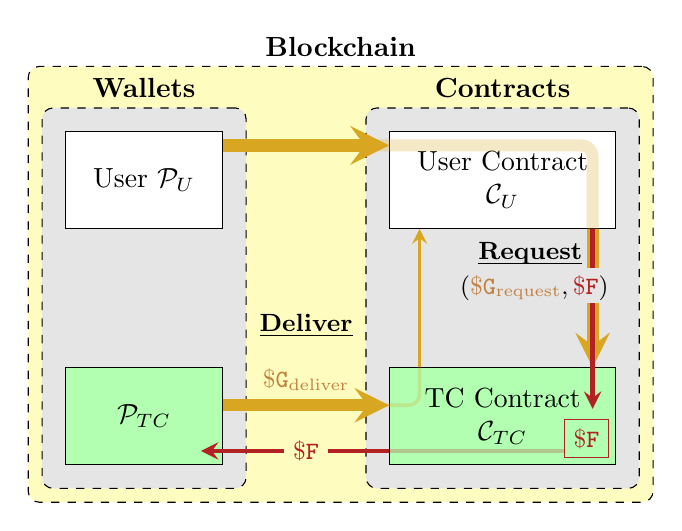
\begin{tikzpicture}
  [contract/.style={entity,minimum height=3.5em,text width=7.5em},
   wallet/.style={entity,minimum height=3.5em,text width=5em},
   type-box-color/.style={fill=black!10},
   blocked-out-label/.style={text=black,type-box-color,text height=0.6em}]
  \node[wallet,fill=white] (user) {User ${\cal P}_U$};
  \node[contract,fill=white,right=6em of user] (cu) {User Contract\\$\reqcont$};
  \node[wallet,trusted,below=5em of user] (tc-wallet) {$\tcadd$};
  \node[contract,trusted,right=6em of tc-wallet] (ctc) {TC Contract\\$\tcont$};
  \node[color=maroon,draw,anchor=south east] (fee) at ([xshift=-0.25em,yshift=0.25em]ctc.south east) {\small $\fee$};

  \draw[color=gold,rounded corners,opacity=0.25,line width=1ex] ([yshift=1.25em]user.east) -| ([xshift=3.25em]cu.south);
  \path[-stealth,color=gold,line width=1.15ex] (user) edge [transform canvas={yshift=1.25em}] (cu);
  \path[-stealth,color=gold,line width=1ex] (cu) edge [transform canvas={xshift=3.25em}] (ctc);
  \path[-stealth,color=maroon,line width=0.4ex] (cu.south) edge [left,transform canvas={xshift=3.25em}] node [blocked-out-label,xshift=1em,yshift=1.2em] {\small \smash{$(\gasrequest, \fee)$}} ([yshift=-1.5em]ctc.north);
  \node[anchor=north,xshift=1em,yshift=-0.75em] () at (cu.south) {\small \bf \underline{\smash{Request}}};

  \path[-stealth,color=gold,line width=1ex] (tc-wallet.east) edge [above,transform canvas={yshift=0.4em}] node () {\small $\gasdeliver$} (ctc.west);
  \draw[color=gold,rounded corners,opacity=0.25,line width=0.3ex] ([yshift=0.4em]tc-wallet.east) -| ([xshift=-3em]ctc.north);
  \path[-stealth,color=gold,line width=0.3ex] (ctc.north) edge [right,transform canvas={xshift=-3em}] node [yshift=-1.25em] {\small \smash{$\gascallback$}} (cu.south);
  \path[color=maroon,opacity=0.25,line width=0.4ex] (tc-wallet-|fee.west) edge [transform canvas={yshift=-1.25em}] (tc-wallet.east);
  \path[-stealth,color=maroon,line width=0.4ex] (ctc.west) edge [transform canvas={yshift=-1.25em}] node [blockchain-color,xshift=0.4em] {\small $\fee$} ([xshift=-0.8em]tc-wallet.east);
%  \path[-stealth,color=gold,ultra thick,dashed] (ctc.west) edge [below,transform canvas={yshift=-1em}] node [text=black,xshift=0.4em] {\small $\gasdeliver - \fee$} ([xshift=-0.8em]tc-wallet.east);

  \path[] (tc-wallet.north east) edge [draw=none,above] node [yshift=0.75em] {\small \bf \underline{Deliver}} (ctc.north west);

  \begin{pgfonlayer}{background}
    \node[bg-box,
          blockchain-color,
          fit={($(ctc.south east)+(1em,-1em)$)($(user.north west)+(-1em,2em)$)},
          label=above:{\bf Blockchain}] () {};
    \node[bg-box,
          type-box-color,
          fit={($(ctc.south east)+(0.5em,-0.5em)$)($(cu.north west)+(-0.5em,0.5em)$)},
          label=above:{\bf Contracts}] () {};
    \node[bg-box,
          type-box-color,
          fit={($(tc-wallet.south east)+(0.5em,-0.5em)$)($(user.north west)+(-0.5em,0.5em)$)},
          label=above:{\bf Wallets}] () {};
  \end{pgfonlayer}
\end{tikzpicture}
\caption{{\bf Blockchain Money Flow within Town Crier.}
Red arrows denote flow of money and brown arrows denote gas provided for function execution.
The thickness of the line indicates the quantity of the resource.
The $\gascallback$ is thin because that value is limited by {\bf Deliver} to $\fee - \constgasmin$.
}
\label{fig:money-flow}
\end{figure}



\paragraph{Town Crier protocol with transaction fees.}
Our basic Town Crier system implements a policy where the requester pays for all gas needed and Town Crier effectively pays nothing.
We now describe how this can be realized by modifying the fee-free protocol described in Section \ethan{refer}.

\begin{itemize}[leftmargin=1.5em]
  \item {\it Initialization.}
    We assume that Town Crier deposits at least $\constgasmax$ into the wallet $\tcadd$.

  \item {\it \tcs blockchain contract.}
    Figure \ref{tbl:tc-contract2} describes the \tcs blockchain contract reflecting fees.
    Since $\tcadd$ must invoke {\bf Deliver}, \tc will pays the gas cost.
    It sets the {\tt GASLIMIT} $\gasdeliver := \constgasmax$.
    To ensure that the gas spent will not exceed the reimbursement available ($\fee$),
    \tcont sets the {\tt GASLIMIT} $\gascallback$ for the sub-call to $\dgcallback$ to $\fee - \constgasmin$.

  \item {\it Town Crier Relay.}
    The relay behavior does not change with the presence of fees.
    It still monitors the blockchain and whenever the contract \tcont stores a new request $(\dgid, \dgform, \_, \_, \_)$,
    it invokes $\enclaveprog$ with $\resumecall(\dgid, \dgform)$.

  \item {\it Town Crier enclave.}
    We make the following small modification to the fee-free protocol.
    Instead of signing the tuple $(\dgid, \dgform, \dgm)$ at the end of its execution,
    the enclave now signs the tuple $(\dgid, \dgform, \dgm, \gasdeliver)$ where $\gasdeliver = \constgasmax$.

  \item {\it Requester.}
    An honest requester behaves the same was as in Figure \ethan{refer} except for setting a {\tt GASLIMIT} of $\gasrequest$ and sending $\fee$ money with each request.
    It sets $\gasrequest$ to be at least the cost of executing the {\bf Request} entry point
    and $\fee$ to be the cost of executing the {\bf Deliver} entry point (including executing the user-defined $\dgcallback$ function).
\end{itemize}

These changes do not modify the properties on which our authenticity proof in Section \ethan{ref authenticity} relied, so that result still holds.
We will prove in Section \ethan{refer} that this new protocol ensures that \tc cannot lose money when the \medname is honest
and that an honest requester's loss is limited even against a malicious \tc.




\subsection{Gas Neutrality}


\begin{theorem}[Gas neutrality for Town Crier]
Assuming an honest Town Crier relay,
Town Crier's wallet account $\tcadd$ will have at least $\constgasmax$ remaining after each {\bf Deliver} call.
\end{theorem}

\begin{proof}[(sketch)]
Honest relay means $\resumecall(\dgid, \dgform)$ will always be legitimate and $\dgform = \dgform'$ in {\bf Deliver}.
While $\fee$ is specified by a potentially malicious user, \tcont rejects the request unless $\constgasmin \leq \fee \leq \constgasmax$.
This means $\gasdeliver = \constgasmax \geq \fee$.
We also will never respond to the same request twice (these are specified in the enclave protocol), so we will never abort.

We limit the gas provided to $\dgcallback$ to $\fee - \constgasmin$ (which must be positive because of the check in {\bf Request}),
and $\constgasmin$ is set so that it is at least the cost of {\bf Deliver} not including $\dgcallback$.
This means that the total gas used is no greater than $\constgasmin + (\fee - \constgasmin) = \fee$, which is exactly what $\tcadd$ is sent for reimbursement.
We also don't run out of gas because $\fee \leq \constgasmax = \gasdeliver$, so we cannot use more gas than we provide.
\end{proof}


\begin{theorem}[Bounded loss for honest requester]
For any request $(\dgform, \dgcallback, \fee)$ submitted by an honest user $\reqcont$,
the requester will lose no more than $\gasrequest + \constgasmax$ money.
\end{theorem}

\begin{proof}[(sketch)]
In Ethereum, all money must be sent by the address controlling that money.
An honest user will only send $\gasrequest + \fee$ to a given request and no more with $\fee \leq \constgasmax$.
They will not continue to send money to \tcont without receiving a response, so that means that they cannot lose more than $\gasrequest + \constgasmax$
even if \tc is malicious and does not deliver data.
\end{proof}






{\footnotesize
  \bibliographystyle{acm}
  \bibliography{ethereum,sgx}
}

%\theendnotes
\end{document}
